\chapter{Related work}\label{chap:related-work}

\section*{}

This chapter presents an overview of the knowledge developed over the years in the areas of industrial robotics, environment perception, machine learning and human-robot interaction that is relevant for the development of cooperative human-robot systems capable of learning and assembling complex objects.


\section{Robotic manipulators}

Robotic manipulators have evolved over the years to fit the automation demand of the industry that required the ability to move the end-effector with accuracy and speed in order to perform a wide range of tasks, which in the case of assembly operations required the capability to sense, grasp and move objects of different size, weight and shape within a given work space. The next sections give a brief overview of the main components of robotic manipulators.


\subsection{Robotic arms}

Robotic arms give the mechanical support for the end effectors (for example grippers, sprayers, grinders, welders, perception sensors, among many others) and can have a wide range of hardware configurations depending on the type of motion that is required for performing a given task. The main categories of robotic arms will be presented in the next sections.


\subsubsection{Cartesian robotic arms}

Cartesian robots have three linear axis of motion (diagrams shown in \cref{fig:cartesian-robot}) and are used in operations that require mainly translations of the end effector (example in \cref{fig:cartesian-robot-festo-3d-gantry}), such as moving objects within large workplaces or spraying / milling / drilling / cutting material using \glspl{cnc} machines.

\begin{figure}[H]
	\begin{floatrow}[2]
		\ffigbox[\FBwidth]
		{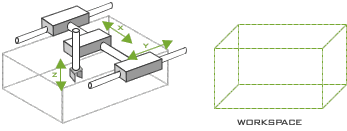
\includegraphics[height=.15\textheight]{robots/cartesian-robot}
		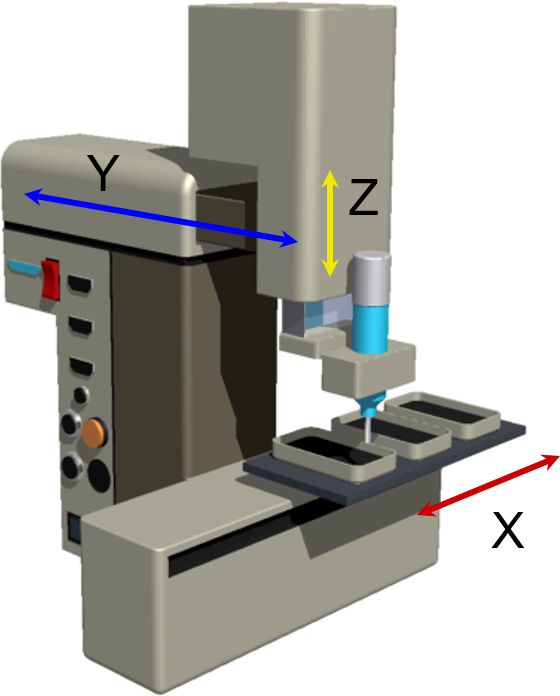
\includegraphics[height=.15\textheight]{robots/cartesian-robot-model}}
		{\caption[Diagrams of a Cartesian robot]{Diagrams of a Cartesian robot\protect\footnotemark}\label{fig:cartesian-robot}}

		\ffigbox[\FBwidth]
		{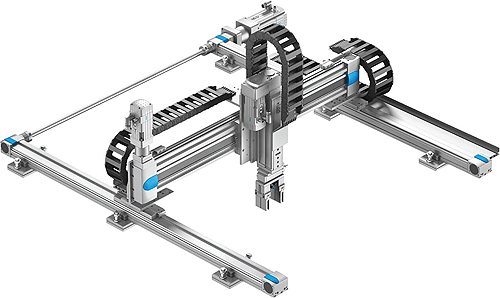
\includegraphics[height=.15\textheight]{robots/cartesian-robot-festo-3d-gantry}}
		{\caption[Cartesian robot with a dual finger gripper]{Cartesian robot with a dual finger gripper\protect\footnotemark}\label{fig:cartesian-robot-festo-3d-gantry}}
	\end{floatrow}
\end{figure}
\footnotetext[\the\numexpr\value{footnote}-1\relax]{\url{http://slideplayer.com/slide/7362200}}
\footnotetext[\value{footnote}]{\url{http://www.linearmotiontips.com/switching-robot-systems-cartesian-handling-systems}}


\subsubsection{Cylindrical robotic arms}

Cylindrical robots have two linear axis and one rotation axis around the origin (diagrams shown in \cref{fig:cylindrical-robot}) and are useful for tasks such as sorting / packaging (example in \cref{fig:cylindrical-robot-plate-crane}) that require the movement of high payload packages.

\begin{figure}[H]
	\begin{floatrow}[2]
		\ffigbox[\FBwidth]
		{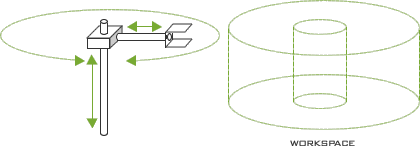
\includegraphics[height=.15\textheight]{robots/cylindrical-robot}
		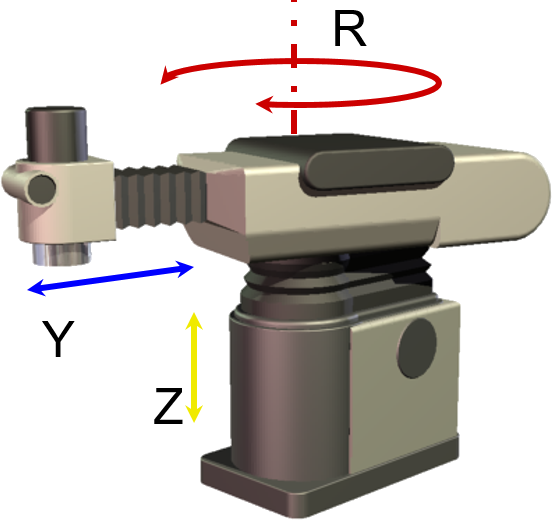
\includegraphics[height=.15\textheight]{robots/cylindrical-robot-model}}
		{\caption[Diagrams of a cylindrical robot]{Diagrams of a cylindrical robot\protect\footnotemark}\label{fig:cylindrical-robot}}

		\ffigbox[\FBwidth]
		{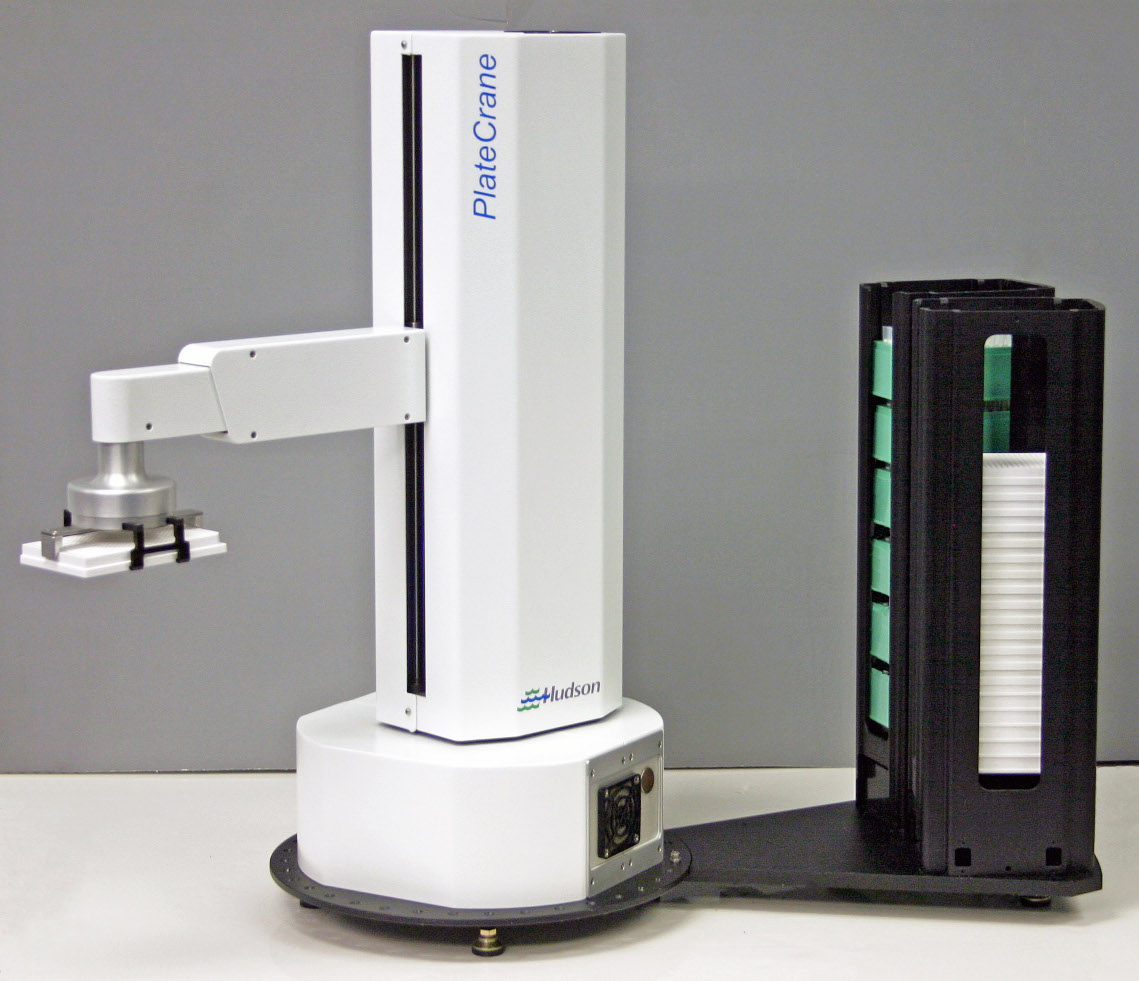
\includegraphics[height=.15\textheight]{robots/cylindrical-robot-plate-crane}}
		{\caption[Cylindrical robot with a dual finger gripper]{Cylindrical robot with a dual finger gripper\protect\footnotemark}\label{fig:cylindrical-robot-plate-crane}}
	\end{floatrow}
\end{figure}
\footnotetext[\the\numexpr\value{footnote}-1\relax]{\url{http://slideplayer.com/slide/7362200}}
\footnotetext[\value{footnote}]{\url{http://hudsonrobotics.com/products/microplate-handling/platecrane-ex}}


\subsubsection{Polar robotic arms}

Polar / spherical robots have one linear axis and two perpendicular rotation axis (diagrams shown in \cref{fig:polar-robot}) and can be used in welding / fettling operations (example in \cref{fig:polar-robot-fanuc}).

\begin{figure}[H]
	\begin{floatrow}[2]
		\ffigbox[\FBwidth]
		{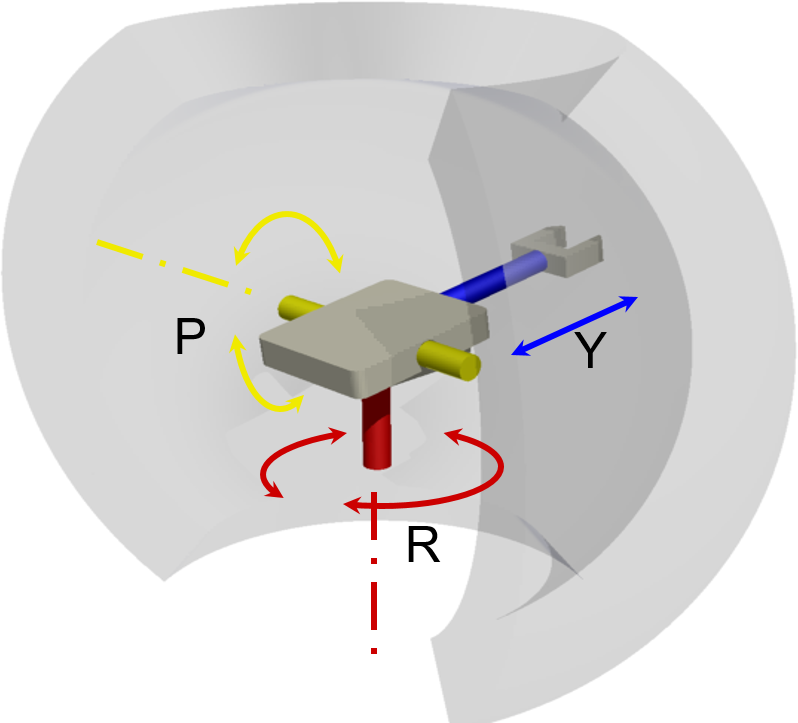
\includegraphics[height=.138\textheight]{robots/polar-robot}
		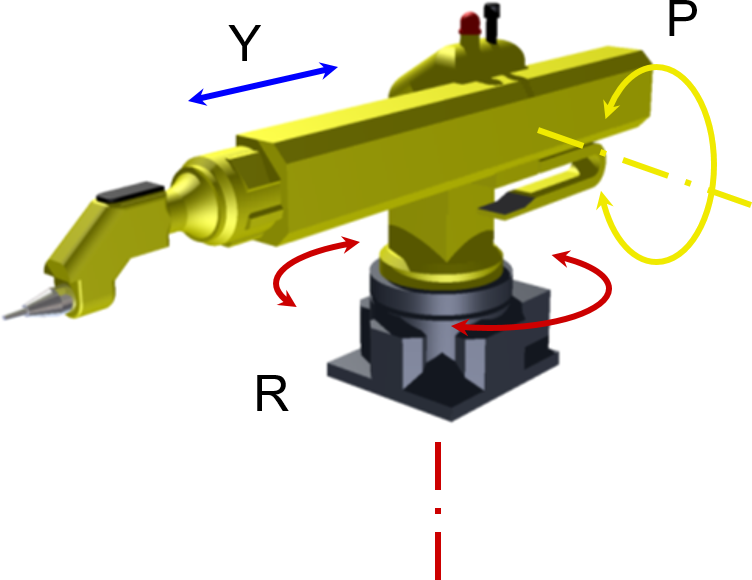
\includegraphics[height=.138\textheight]{robots/polar-robot-model}}
		{\caption[Diagrams of a polar robot]{Diagrams of a polar robot\protect\footnotemark}\label{fig:polar-robot}}

		\ffigbox[\FBwidth]
		{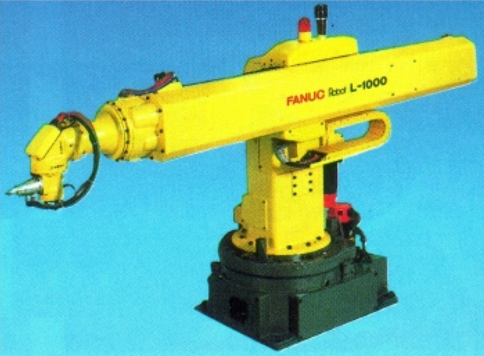
\includegraphics[height=.138\textheight]{robots/polar-robot-fanuc}}
		{\caption[Polar robot]{Polar robot\protect\footnotemark}\label{fig:polar-robot-fanuc}}
	\end{floatrow}
\end{figure}
\footnotetext[\the\numexpr\value{footnote}-1\relax]{\url{http://slideplayer.com/slide/7362200}}
\footnotetext[\value{footnote}]{\url{http://saba.kntu.ac.ir/eecd/ecourses/robotics/overview.pdf}}


\subsubsection{\glsentrytext{scara} robotic arms}

\gls{scara} robots have one linear axis and two parallel rotation axis (diagrams shown in \cref{fig:scara-robot}) and can perform quick pick and place tasks (example in \cref{fig:scara-robot-packaging}).

\begin{figure}[H]
	\begin{floatrow}[2]
		\ffigbox[\FBwidth]
		{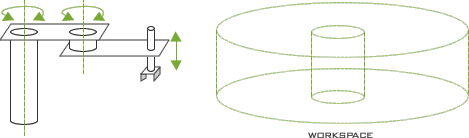
\includegraphics[height=.173\textheight]{robots/scara-robot}
		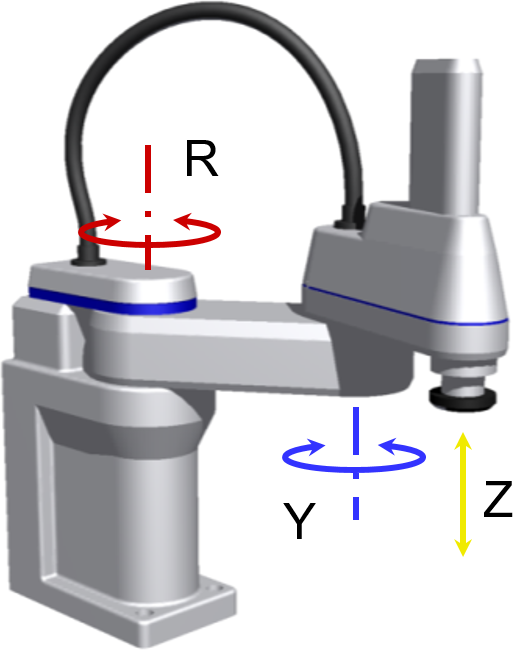
\includegraphics[height=.173\textheight]{robots/scara-robot-model}}
		{\caption[Diagrams of a \glsentrytext{scara} robot]{Diagrams of a \glsentrytext{scara} robot\protect\footnotemark}\label{fig:scara-robot}}

		\ffigbox[\FBwidth]
		{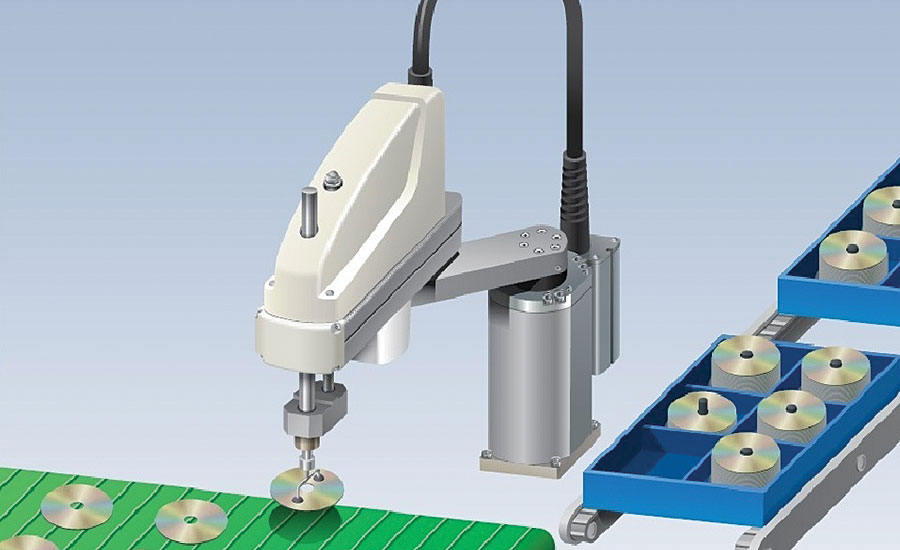
\includegraphics[height=.173\textheight]{robots/scara-robot-packaging}}
		{\caption[\glsentrytext{scara} robot packaging products]{\glsentrytext{scara} robot packaging products\protect\footnotemark}\label{fig:scara-robot-packaging}}
	\end{floatrow}
\end{figure}
\footnotetext[\the\numexpr\value{footnote}-1\relax]{\url{http://slideplayer.com/slide/7362200}}
\footnotetext[\value{footnote}]{\url{http://www.assemblymag.com/articles/93338-whats-new-with-scara-robots}}


\subsubsection{Parallel / delta robotic arms}

Picker / delta / parallel robots have three parallelogram arms connected to the end effector in order to provide three translation axis and one rotation axis (diagrams shown in \cref{fig:schema-delta-type-1-side-view,fig:paralell-robot-abb}) and they can perform very fast pick and place tasks (example in \cref{fig:picker-parallel-robot-fanuc}).

\begin{figure}[H]
	\begin{floatrow}[3]
		\ffigbox[1.05\FBwidth]
		{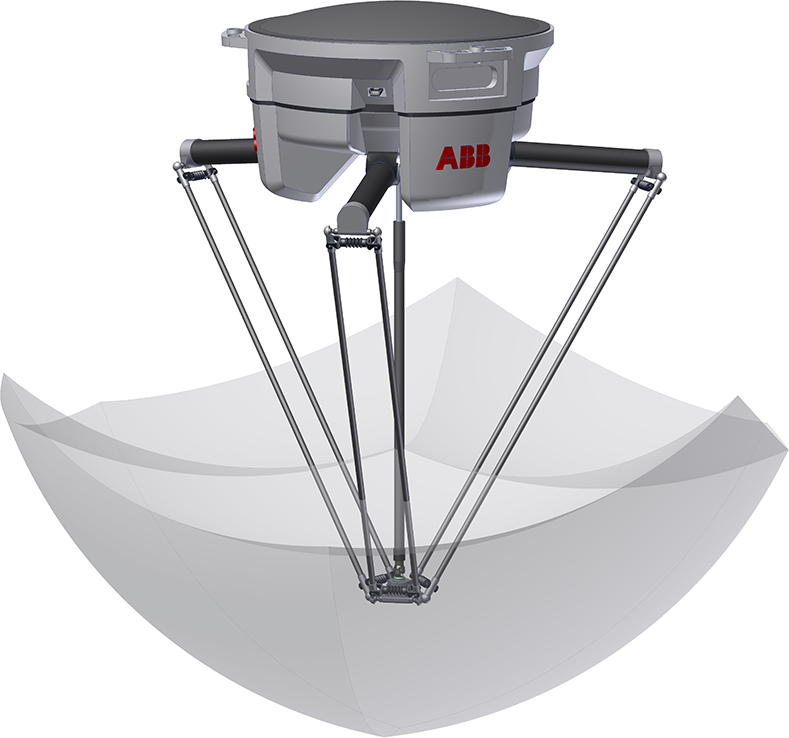
\includegraphics[height=.205\textheight]{robots/paralell-robot-abb}}
		{\caption[Model of a delta robot]{Model of a delta robot\protect\footnotemark}\label{fig:paralell-robot-abb}}

		\ffigbox[\FBwidth]
		{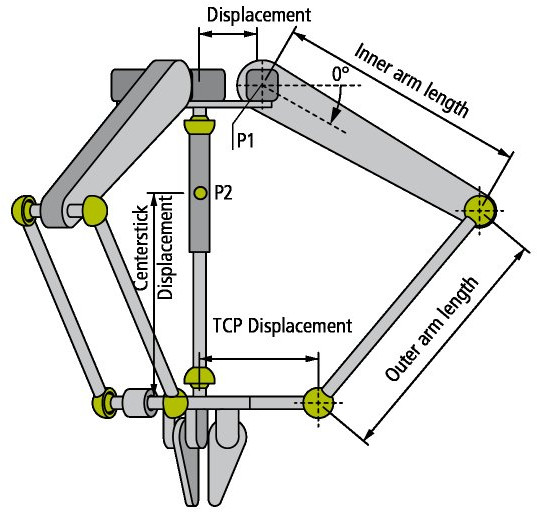
\includegraphics[height=.205\textheight]{robots/schema-delta-type-1-side-view}}
		{\caption[Diagram of a delta robot]{Diagram of a delta robot\protect\footnotemark}\label{fig:schema-delta-type-1-side-view}}

		\ffigbox[\FBwidth]
		{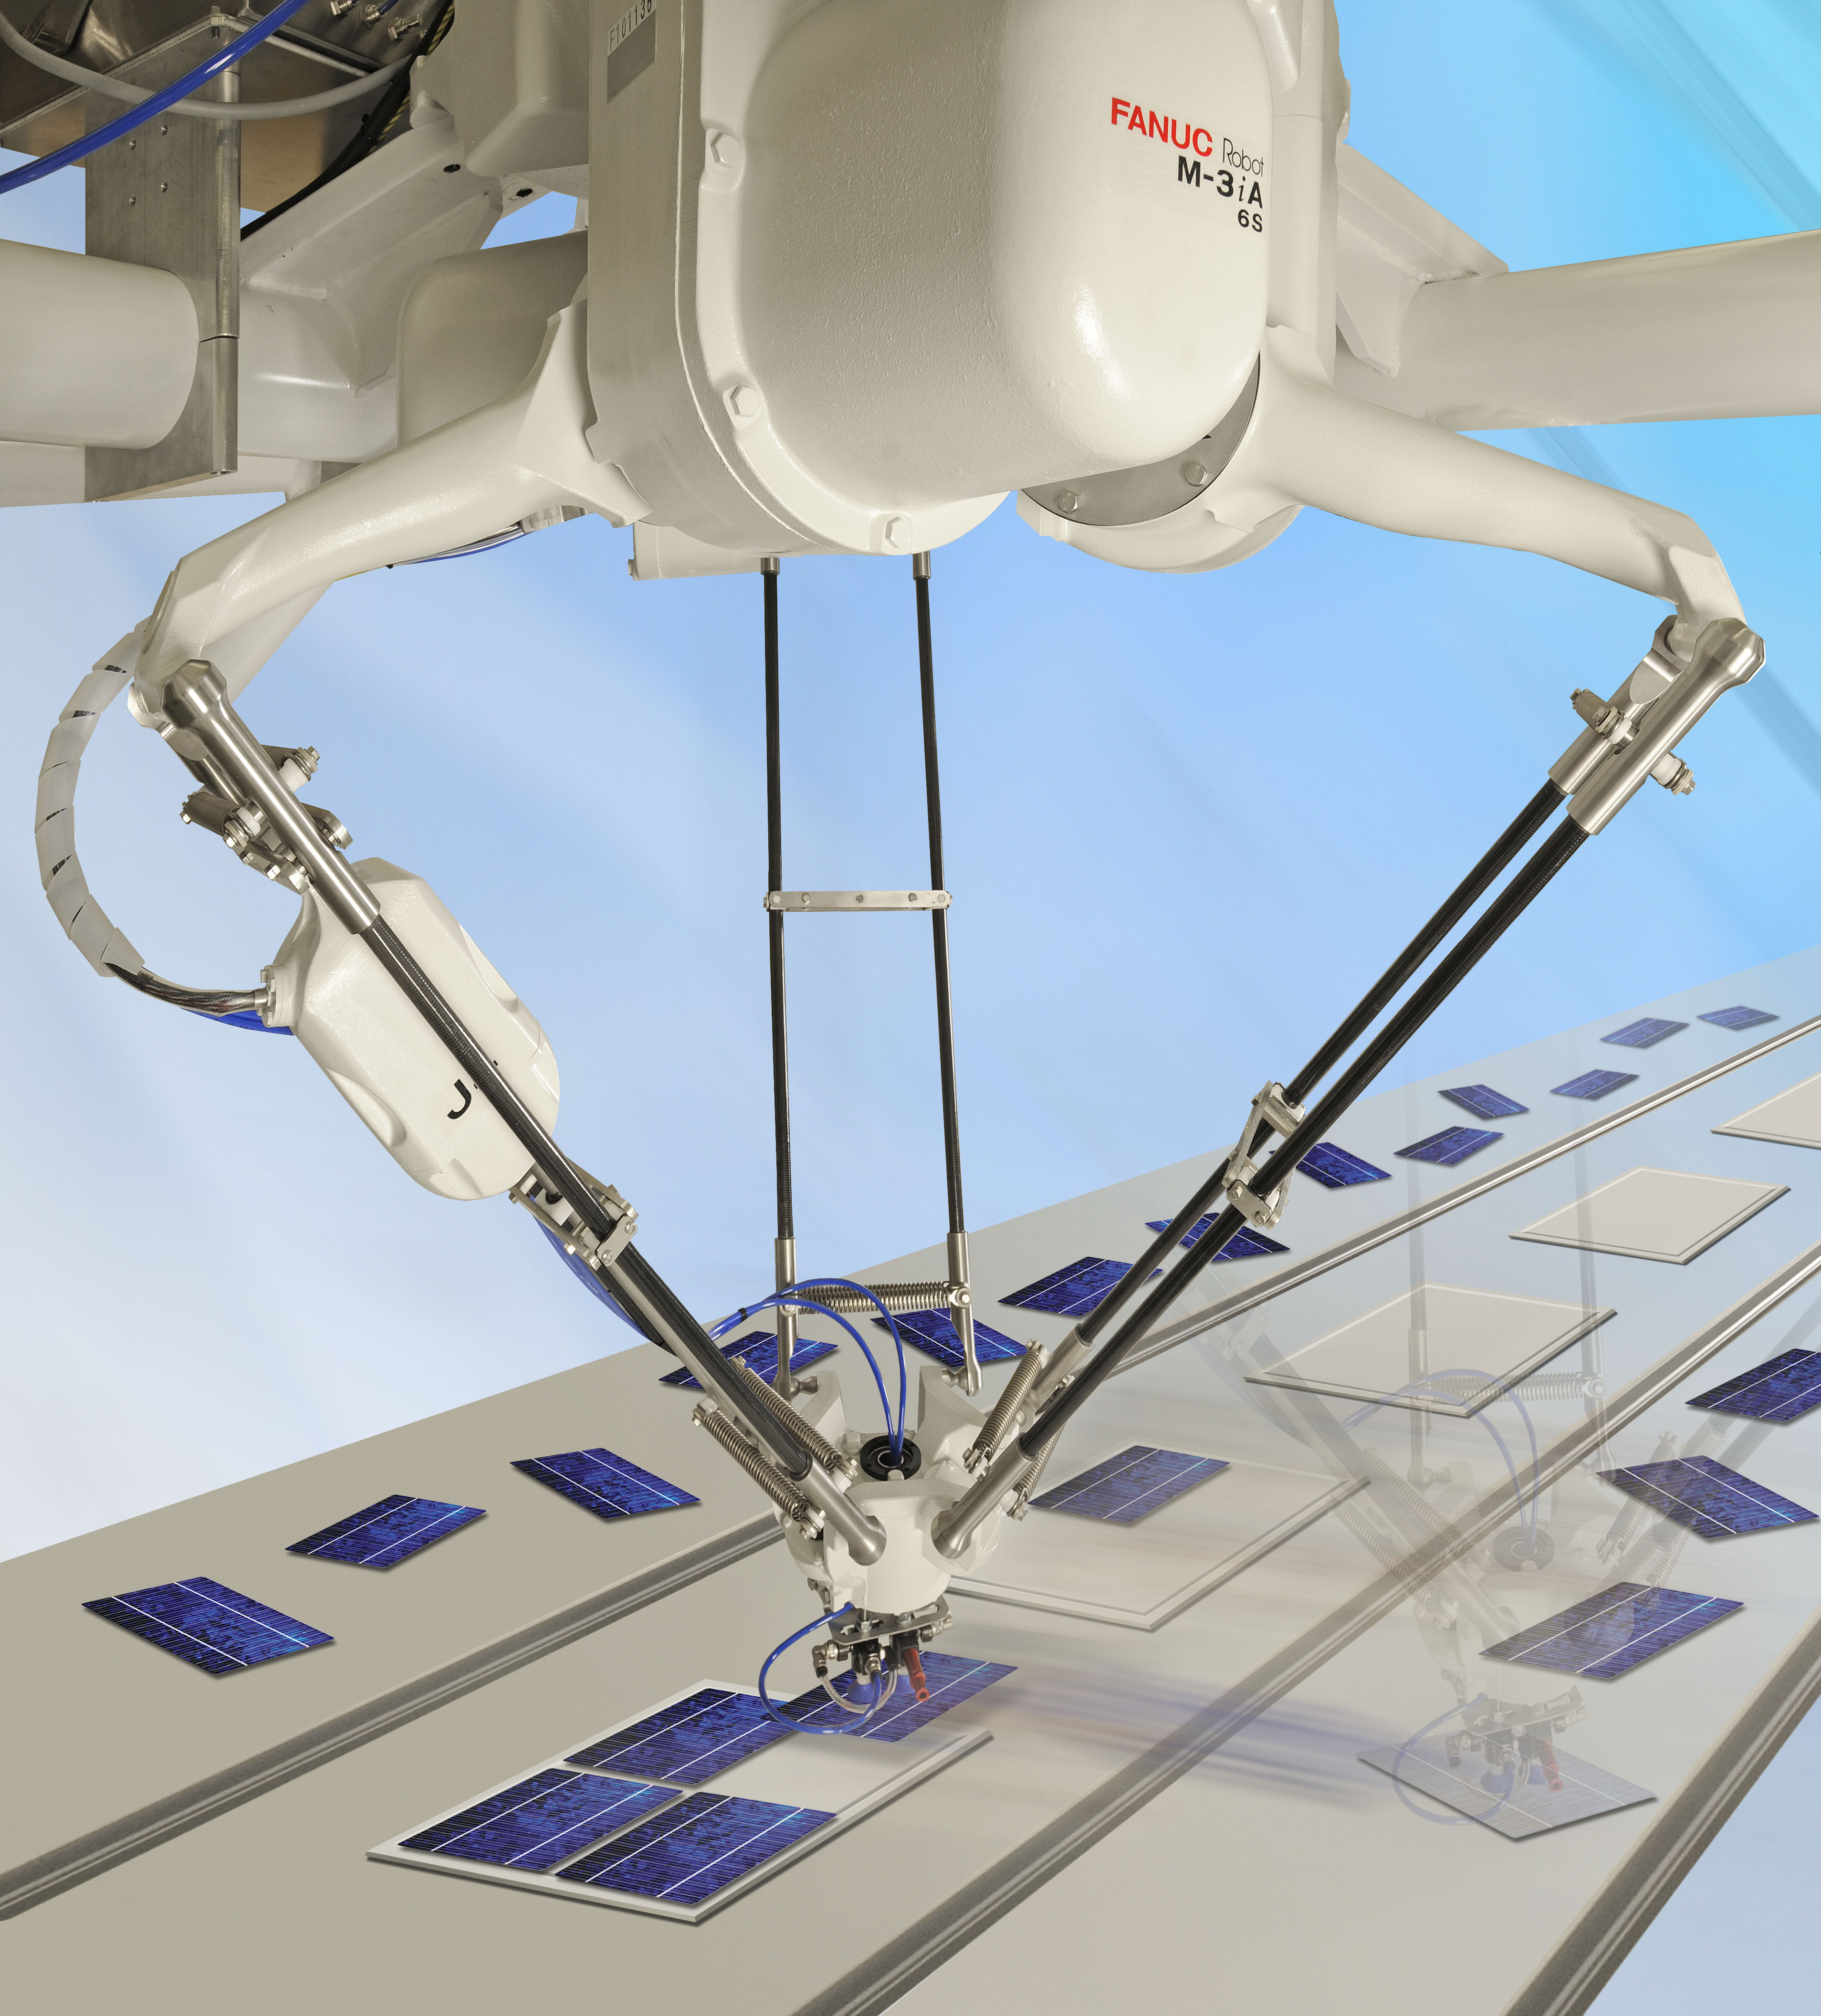
\includegraphics[height=.205\textheight]{robots/picker-parallel-robot-fanuc}}
		{\caption[Delta robot packaging products]{Delta robot packaging products\protect\footnotemark}\label{fig:picker-parallel-robot-fanuc}}
	\end{floatrow}
\end{figure}
\footnotetext[\the\numexpr\value{footnote}-2\relax]{\url{http://www.mecademic.com/What-is-a-parallel-robot.html}}
\footnotetext[\the\numexpr\value{footnote}-1\relax]{\url{http://infosys.beckhoff.com/content/1034/tckintransformation/html/tcnckintransformation_deltatype1.htm?id=21945}}
\footnotetext[\value{footnote}]{\url{http://robot.fanucamerica.com/products/robots/picking-and-packing-robots.aspx}}


\subsubsection{Snake robotic arms}

Snake robots are flexible manipulators with a high number of interconnected joints (structure of a snake robot shown in \cref{fig:snake-arm-robot-diagram}) capable of bending like a snake in order to access small and difficult to reach areas (example in \cref{fig:laser-snake-pipe-cutting}).


\begin{figure}[H]
	\begin{floatrow}[2]
		\ffigbox[\FBwidth]
		{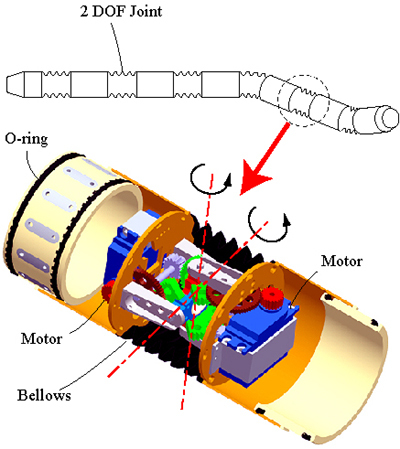
\includegraphics[height=.173\textheight]{robots/snake-robot-diagram}
		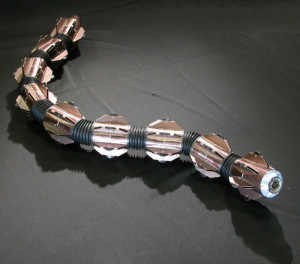
\includegraphics[height=.173\textheight]{robots/snake-robot}}
		{\caption[Structure of a snake robot]{Structure of a snake robot\protect\footnotemark}\label{fig:snake-arm-robot-diagram}}

		\ffigbox[\FBwidth]
		{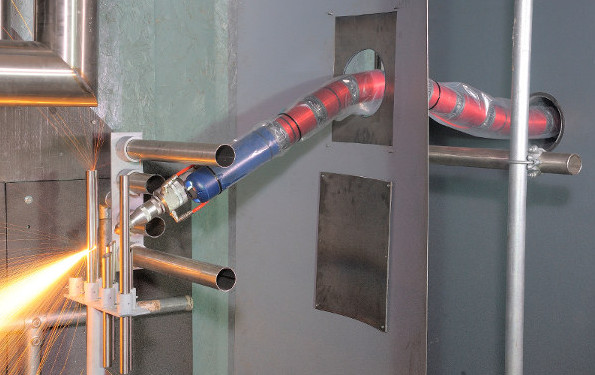
\includegraphics[height=.173\textheight]{robots/laser-snake-pipe-cutting}}
		{\caption[Laser snake robot cutting a pipe]{Laser snake robot cutting a pipe\protect\footnotemark}\label{fig:laser-snake-pipe-cutting}}
	\end{floatrow}
\end{figure}
\footnotetext[\the\numexpr\value{footnote}-1\relax]{\url{https://techcrunch.com/2010/08/18/video-giant-snake-robot-acm-r5}}
\footnotetext[\value{footnote}]{\url{http://sparc-robotics.eu/nuclear-decommissioning}}


\subsubsection{Articulated robotic arms}

Articulated robots are versatile arms with at least 3 rotation axis (diagrams shown in \cref{fig:articulated-robot}) and are capable of performing a wide range of tasks, from welding to advanced assembly tasks (example in \cref{fig:articulated-robot-kuka}).

\begin{figure}[H]
	\begin{floatrow}[2]
		\ffigbox[\FBwidth]
		{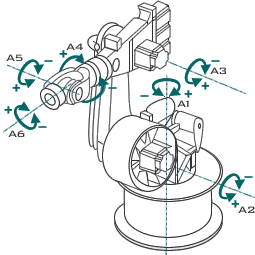
\includegraphics[height=.187\textheight]{robots/articulated-robot}
		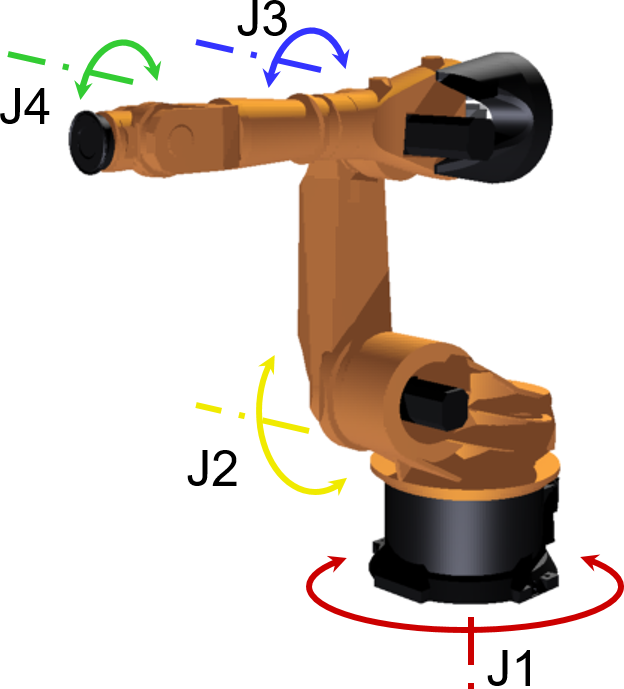
\includegraphics[height=.187\textheight]{robots/articulated-robot-model}}
		{\caption[Diagrams of an articulated robot]{Diagrams of an articulated robot\protect\footnotemark}\label{fig:articulated-robot}}

		\ffigbox[\FBwidth]
		{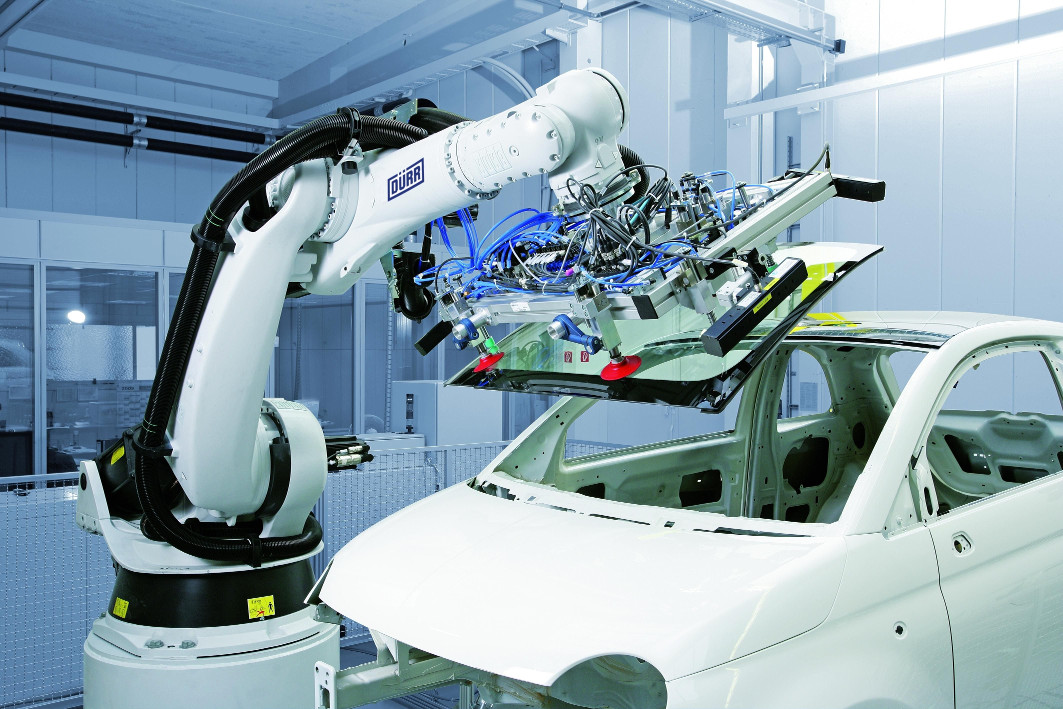
\includegraphics[height=.187\textheight]{robots/articulated-robot-kuka}}
		{\caption[Articulated  robot installing a windshield in a car]{Articulated  robot installing a windshield in a car\protect\footnotemark}\label{fig:articulated-robot-kuka}}
	\end{floatrow}
\end{figure}
\footnotetext[\the\numexpr\value{footnote}-1\relax]{\url{http://slideplayer.com/slide/7362200}}
\footnotetext[\value{footnote}]{\url{http://gracemarketdata.com/index.php/component/virtuemart/2001-detail}}



\subsubsection{Collaborative robotic arms}

Collaborative robots are usually articulated robotic arms that were designed to be safe to operate around humans. They typically move at low velocities and have force-torque / motor current sensors along with enclosure in pressure / capacitive sensitive materials in order to detect collisions and stop the robot movement before injuring humans. Other safety measures rely on the usage of elastic actuators and soft padding to attenuate the impact damage while complementary measures include the detection of approaching humans / objects using \glspl{lidar} / RGB-D sensors in order to reduce the robot operation velocity and adjust the trajectory to avoid collisions. In \cref{fig:collaborative-robots-t1,fig:collaborative-robots-t2} it is presented an overview of the main collaborative robots currently available along with the specification of their main hardware characteristics and targeted applications.

%Articles:\\
%- Collaborative robot - Robotiq ebook | Mathieu2015
%- Dual arm manipulation - A survey | Smith2012
%- A brief survey of commercial robotic arms for research on manipulation | Lu2012
%- Survey of robotic arm and parameters | Patidar2016


\begin{table}[H]
	\centering
	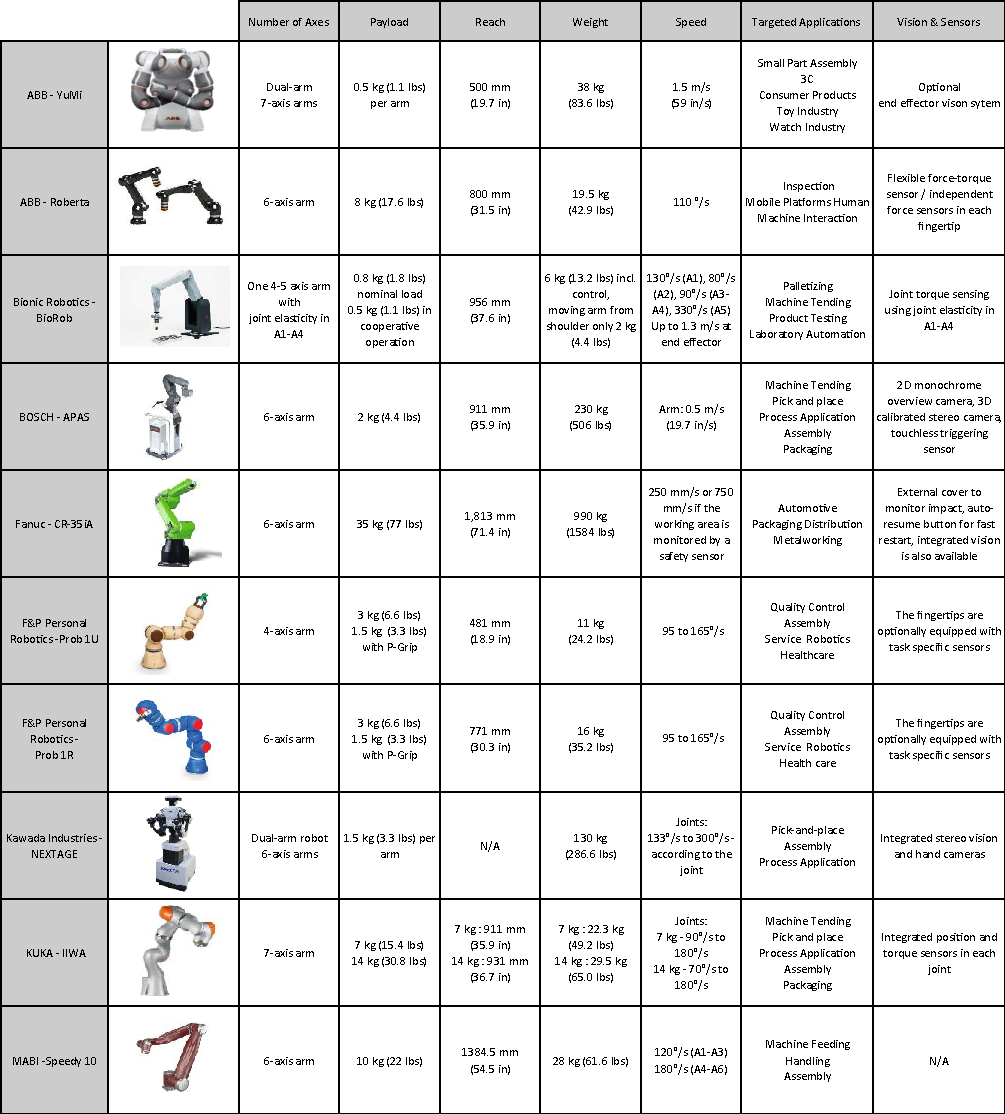
\includegraphics[width=\linewidth]{robots/collaborative-robots-t1}
	\caption[Collaborative robots (a)]{Collaborative robots (a) \cite{Mathieu2015}}
	\label{fig:collaborative-robots-t1}
\end{table}

\begin{table}[H]
	\centering
	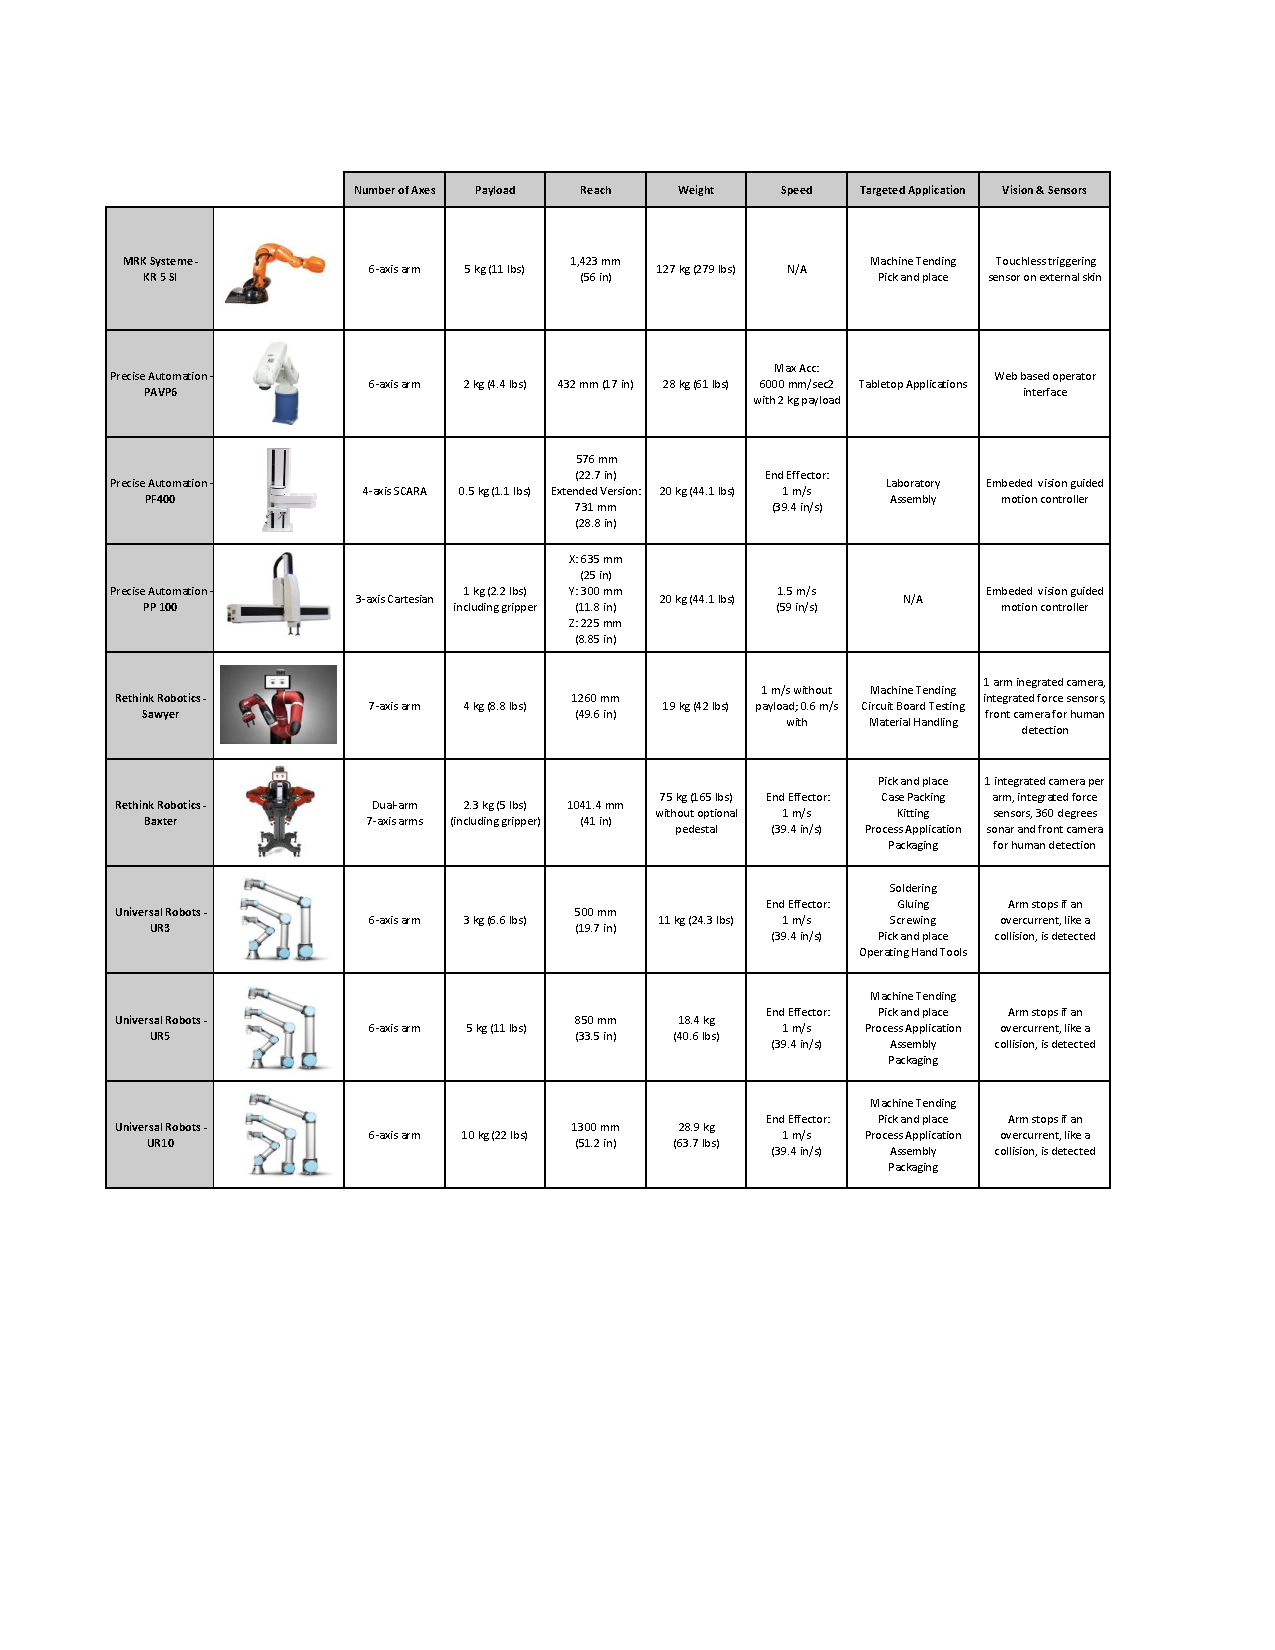
\includegraphics[width=\linewidth]{robots/collaborative-robots-t2}
	\caption[Collaborative robots (b)]{Collaborative robots (b) \cite{Mathieu2015}}
	\label{fig:collaborative-robots-t2}
\end{table}


\subsection{Robotic end effectors}

End effectors are hardware devices attached at the end of robotic arms in order to allow them to interact with the environment. This interaction can be passive if the end effectors are only comprised of sensors (used for inspection, quality assurance, surveillance) or can be active in which the robot physically interacts with the environment.

Grippers are one the most complex active end effectors given their need to grasp and hold a wide range of objects with different size, shape, weight and stiffness. They are also one of the most flexible and versatile end effector given that they can be used to handle a wide range of objects when performing very different tasks. The remaining end effectors are usually tailored for very specific tasks (for example welding, cutting, drilling, screwing, grinding, painting, among many others).

The following list presents a brief overview of the main end effectors currently available.

\begin{itemize}
	\item Grippers
	\begin{itemize}
		\item Impactive grippers
		\begin{itemize}
			\item Parallel fingers
			\item Angular fingers
			\item Universal grippers (for example the Versaball)
			\item Anthropomorphic grippers with 5 fingers
		\end{itemize}
		\item Astrictive grippers
		\begin{itemize}
			\item Vacuum grippers
			\item Bernoulli grippers
			\item Magnetic grippers
			\item Electrostatic grippers
		\end{itemize}
		\item Contigutive grippers
		\begin{itemize}
			\item Chemical adhesion grippers
			\item Thermal adhesion grippers
		\end{itemize}
		\item Ingressive grippers
		\begin{itemize}
			\item Hooks
			\item Loops
		\end{itemize}
	\end{itemize}
	\item Perception sensors
	\begin{itemize}
		\item 2D / \gls{tof} cameras
		\item Point / line lasers
		\item \glspl{lidar}
		\item RGB-D sensors
		\item Structured light sensors
	\end{itemize}
	\item Collision sensors
	\item Force-torque sensors
	\item Projectors (\gls{dlp} / galvanometers)
	\item Welding torches
	\item Cutting tools
	\item Drilling tools
	\item Milling tools
	\item Grinders
	\item Sanders
	\item Polishers
	\item Finishers
	\item Sprayers
	\item Screw drivers
	\item Spanners
	\item Ladles
\end{itemize}


For assembly operations the most useful end effectors are the grippers, perception / force-torque sensors and specialized tools (screw drivers, spanners, welders, among others). Most object manipulation tasks can be done with grippers with two or three fingers (examples in \cref{fig:yumi-gripper-vamera-vacuum,fig:schunk-parallel-grippers,fig:schunk-angular-gripper,fig:schunk-self-centering-gripper}) or with adaptive two / three finger grippers (examples in \cref{fig:robotiq-adaptive-2-finger-gripper,fig:robotiq-adaptive-3-finger-gripper}). For tasks that require coarse accuracy, magnetic / vacuum grippers (examples in \cref{fig:zimmer-magnetic-gripper,fig:schunk-vacuum-gripper,fig:schmalz-vacuum-area-gripper}) might be a suitable alternative. For difficult to grasp objects, flexible grippers (such as the ones shown in \cref{fig:versa-ball,fig:festo-multichoice-gripper}) provide a robust approach. For very complex tasks that may require advanced dexterity, anthropomorphic grippers (example in \cref{fig:schunk-svh-hand}) offer a very advanced solution.

\begin{figure}[H]
	\begin{floatrow}[4]
		\ffigbox[1.1\FBwidth]
		{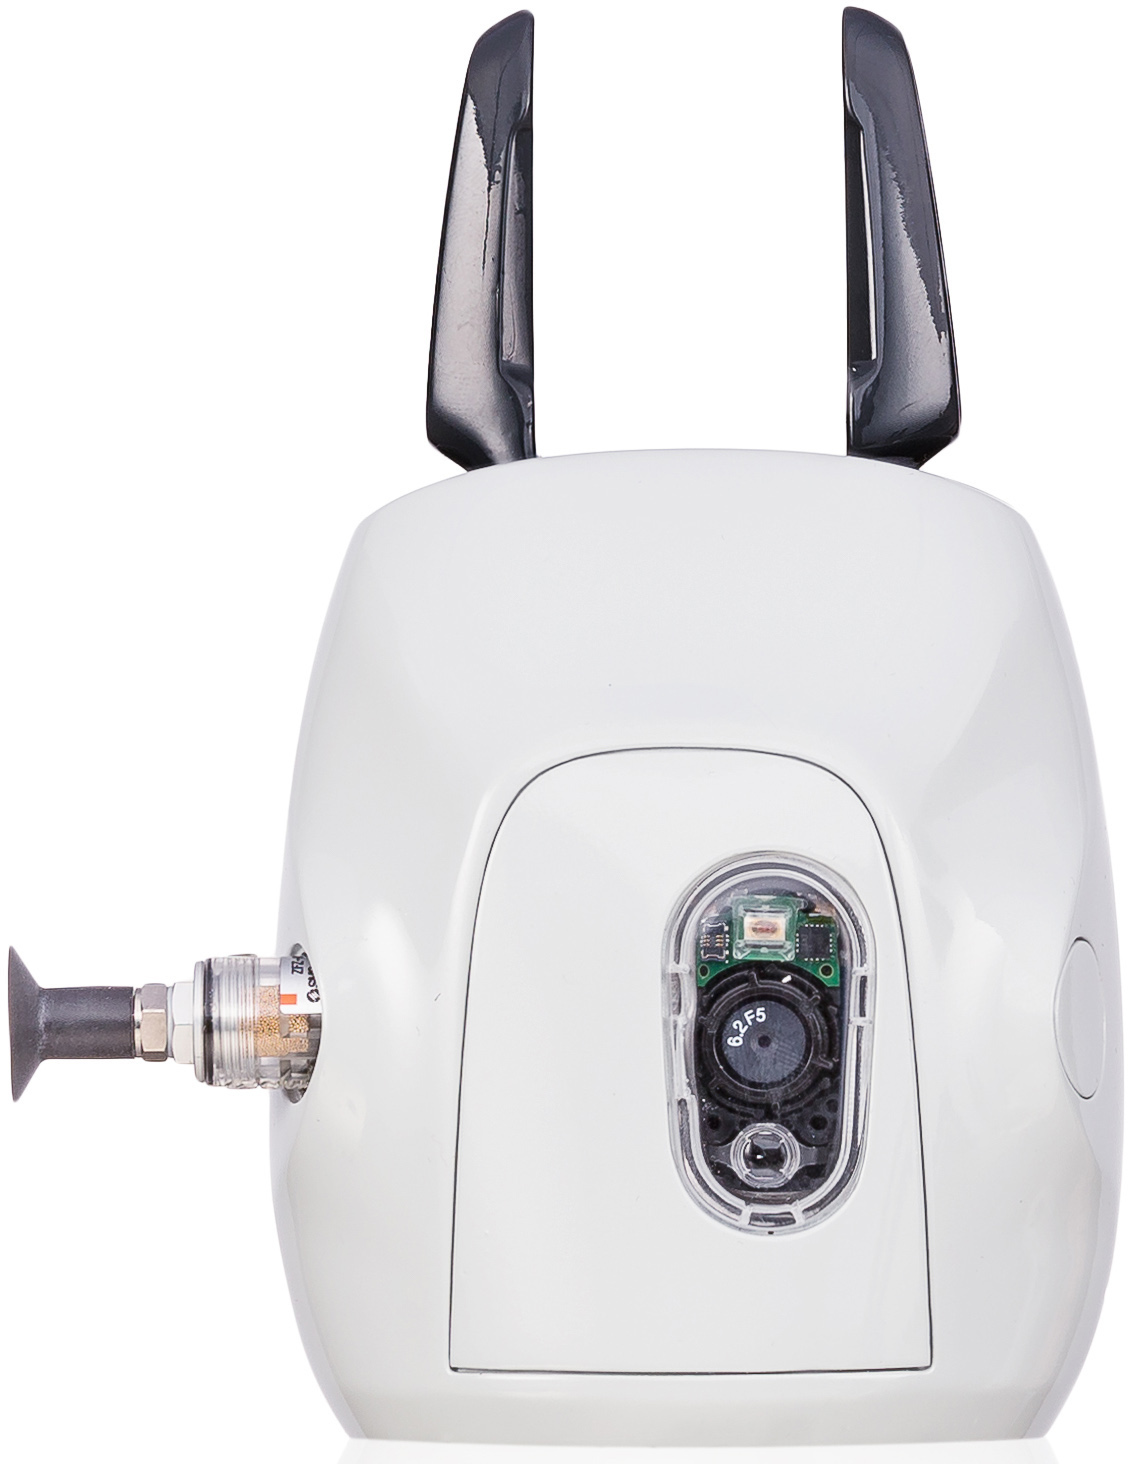
\includegraphics[height=.19\textheight]{grippers/yumi-gripper-vamera-vacuum}}
		{\caption[ABB Yumi dual finger / vacuum / camera gripper]{ABB Yumi dual finger / vacuum / camera gripper \protect\footnotemark}\label{fig:yumi-gripper-vamera-vacuum}}

		\ffigbox[1.1\FBwidth]
		{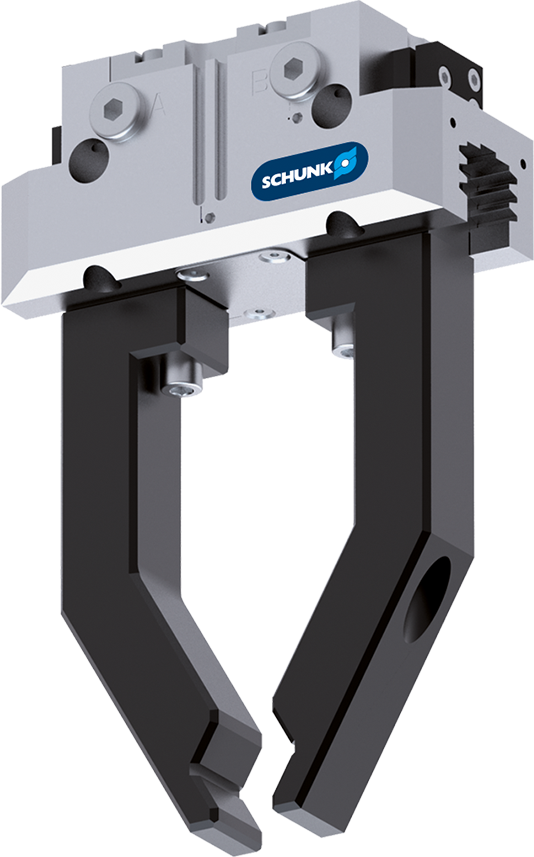
\includegraphics[height=.19\textheight]{grippers/schunk-parallel}}
		{\caption[Schunk parallel gripper]{Schunk parallel gripper\protect\footnotemark}\label{fig:schunk-parallel-grippers}}

		\ffigbox[1.1\FBwidth]
		{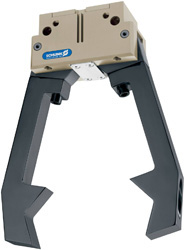
\includegraphics[height=.19\textheight]{grippers/schunk-angular-gripper}}
		{\caption[Schunk angular gripper]{Schunk angular gripper\protect\footnotemark}\label{fig:schunk-angular-gripper}}

		\ffigbox[1.1\FBwidth]
		{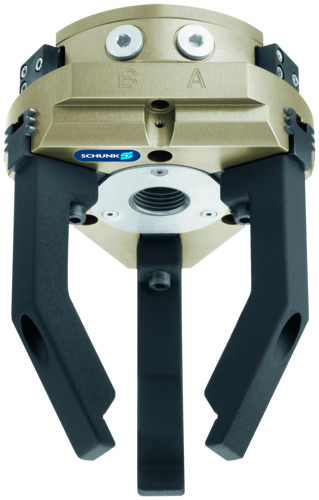
\includegraphics[height=.19\textheight]{grippers/schunk-self-centering-gripper}}
		{\caption[Schunk self-centering gripper]{Schunk self-centering gripper\protect\footnotemark}\label{fig:schunk-self-centering-gripper}}
	\end{floatrow}
\end{figure}
\footnotetext[\the\numexpr\value{footnote}-3\relax]{\url{http://new.abb.com/products/robotics/yumi}}
\footnotetext[\the\numexpr\value{footnote}-2\relax]{\url{https://us.schunk.com/us_en/home/pgn-plus-p}}
\footnotetext[\the\numexpr\value{footnote}-1\relax]{\url{https://us.schunk.com/us_en/gripping-systems/\#/series/pwg-plus}}
\footnotetext[\value{footnote}]{\url{https://us.schunk.com/us_en/gripping-systems/\#/series/pzb-plus}}


\begin{figure}[H]
	\begin{floatrow}[4]
		\ffigbox[1.05\FBwidth]
		{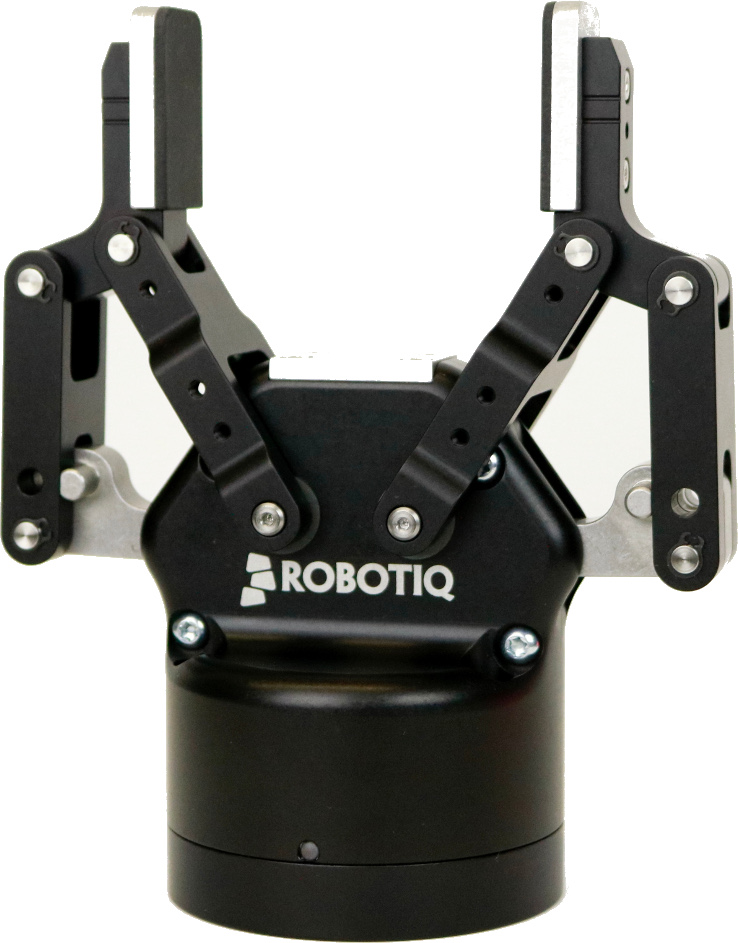
\includegraphics[height=.17\textheight]{grippers/robotiq-adaptive-2-finger-gripper}}
		{\caption[Robotiq adaptive 2 finger gripper]{Robotiq adaptive 2 finger gripper\protect\footnotemark}\label{fig:robotiq-adaptive-2-finger-gripper}}

		\ffigbox[1.05\FBwidth]
		{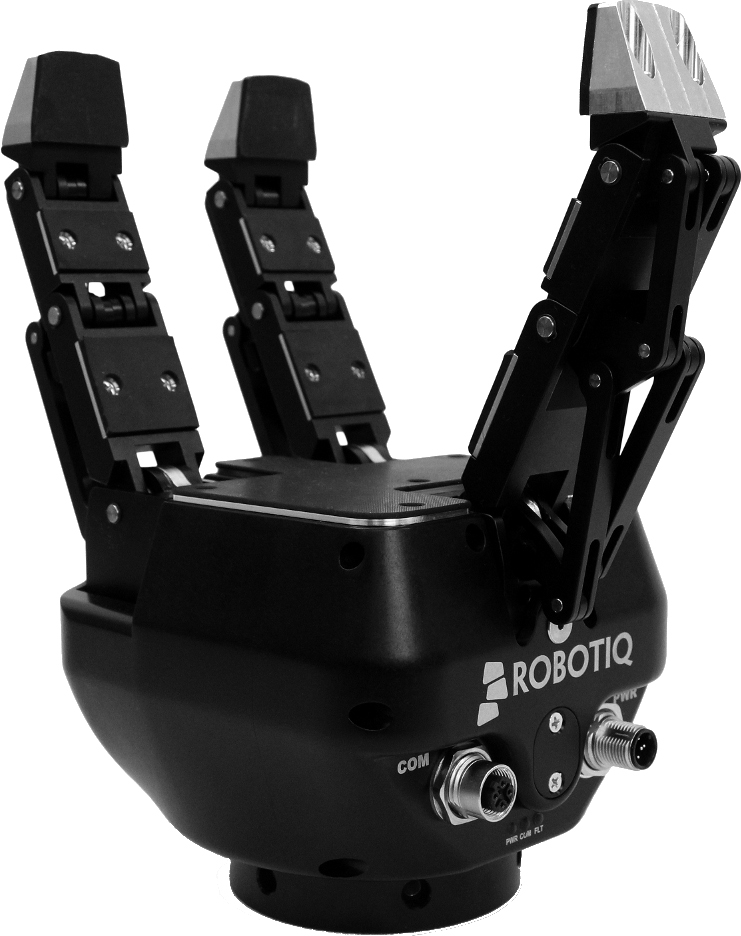
\includegraphics[height=.17\textheight]{grippers/robotiq-adaptive-3-finger-gripper}}
		{\caption[Robotiq adaptive 3 finger gripper]{Robotiq adaptive 3 finger gripper\protect\footnotemark}\label{fig:robotiq-adaptive-3-finger-gripper}}

		\ffigbox[1.05\FBwidth]
		{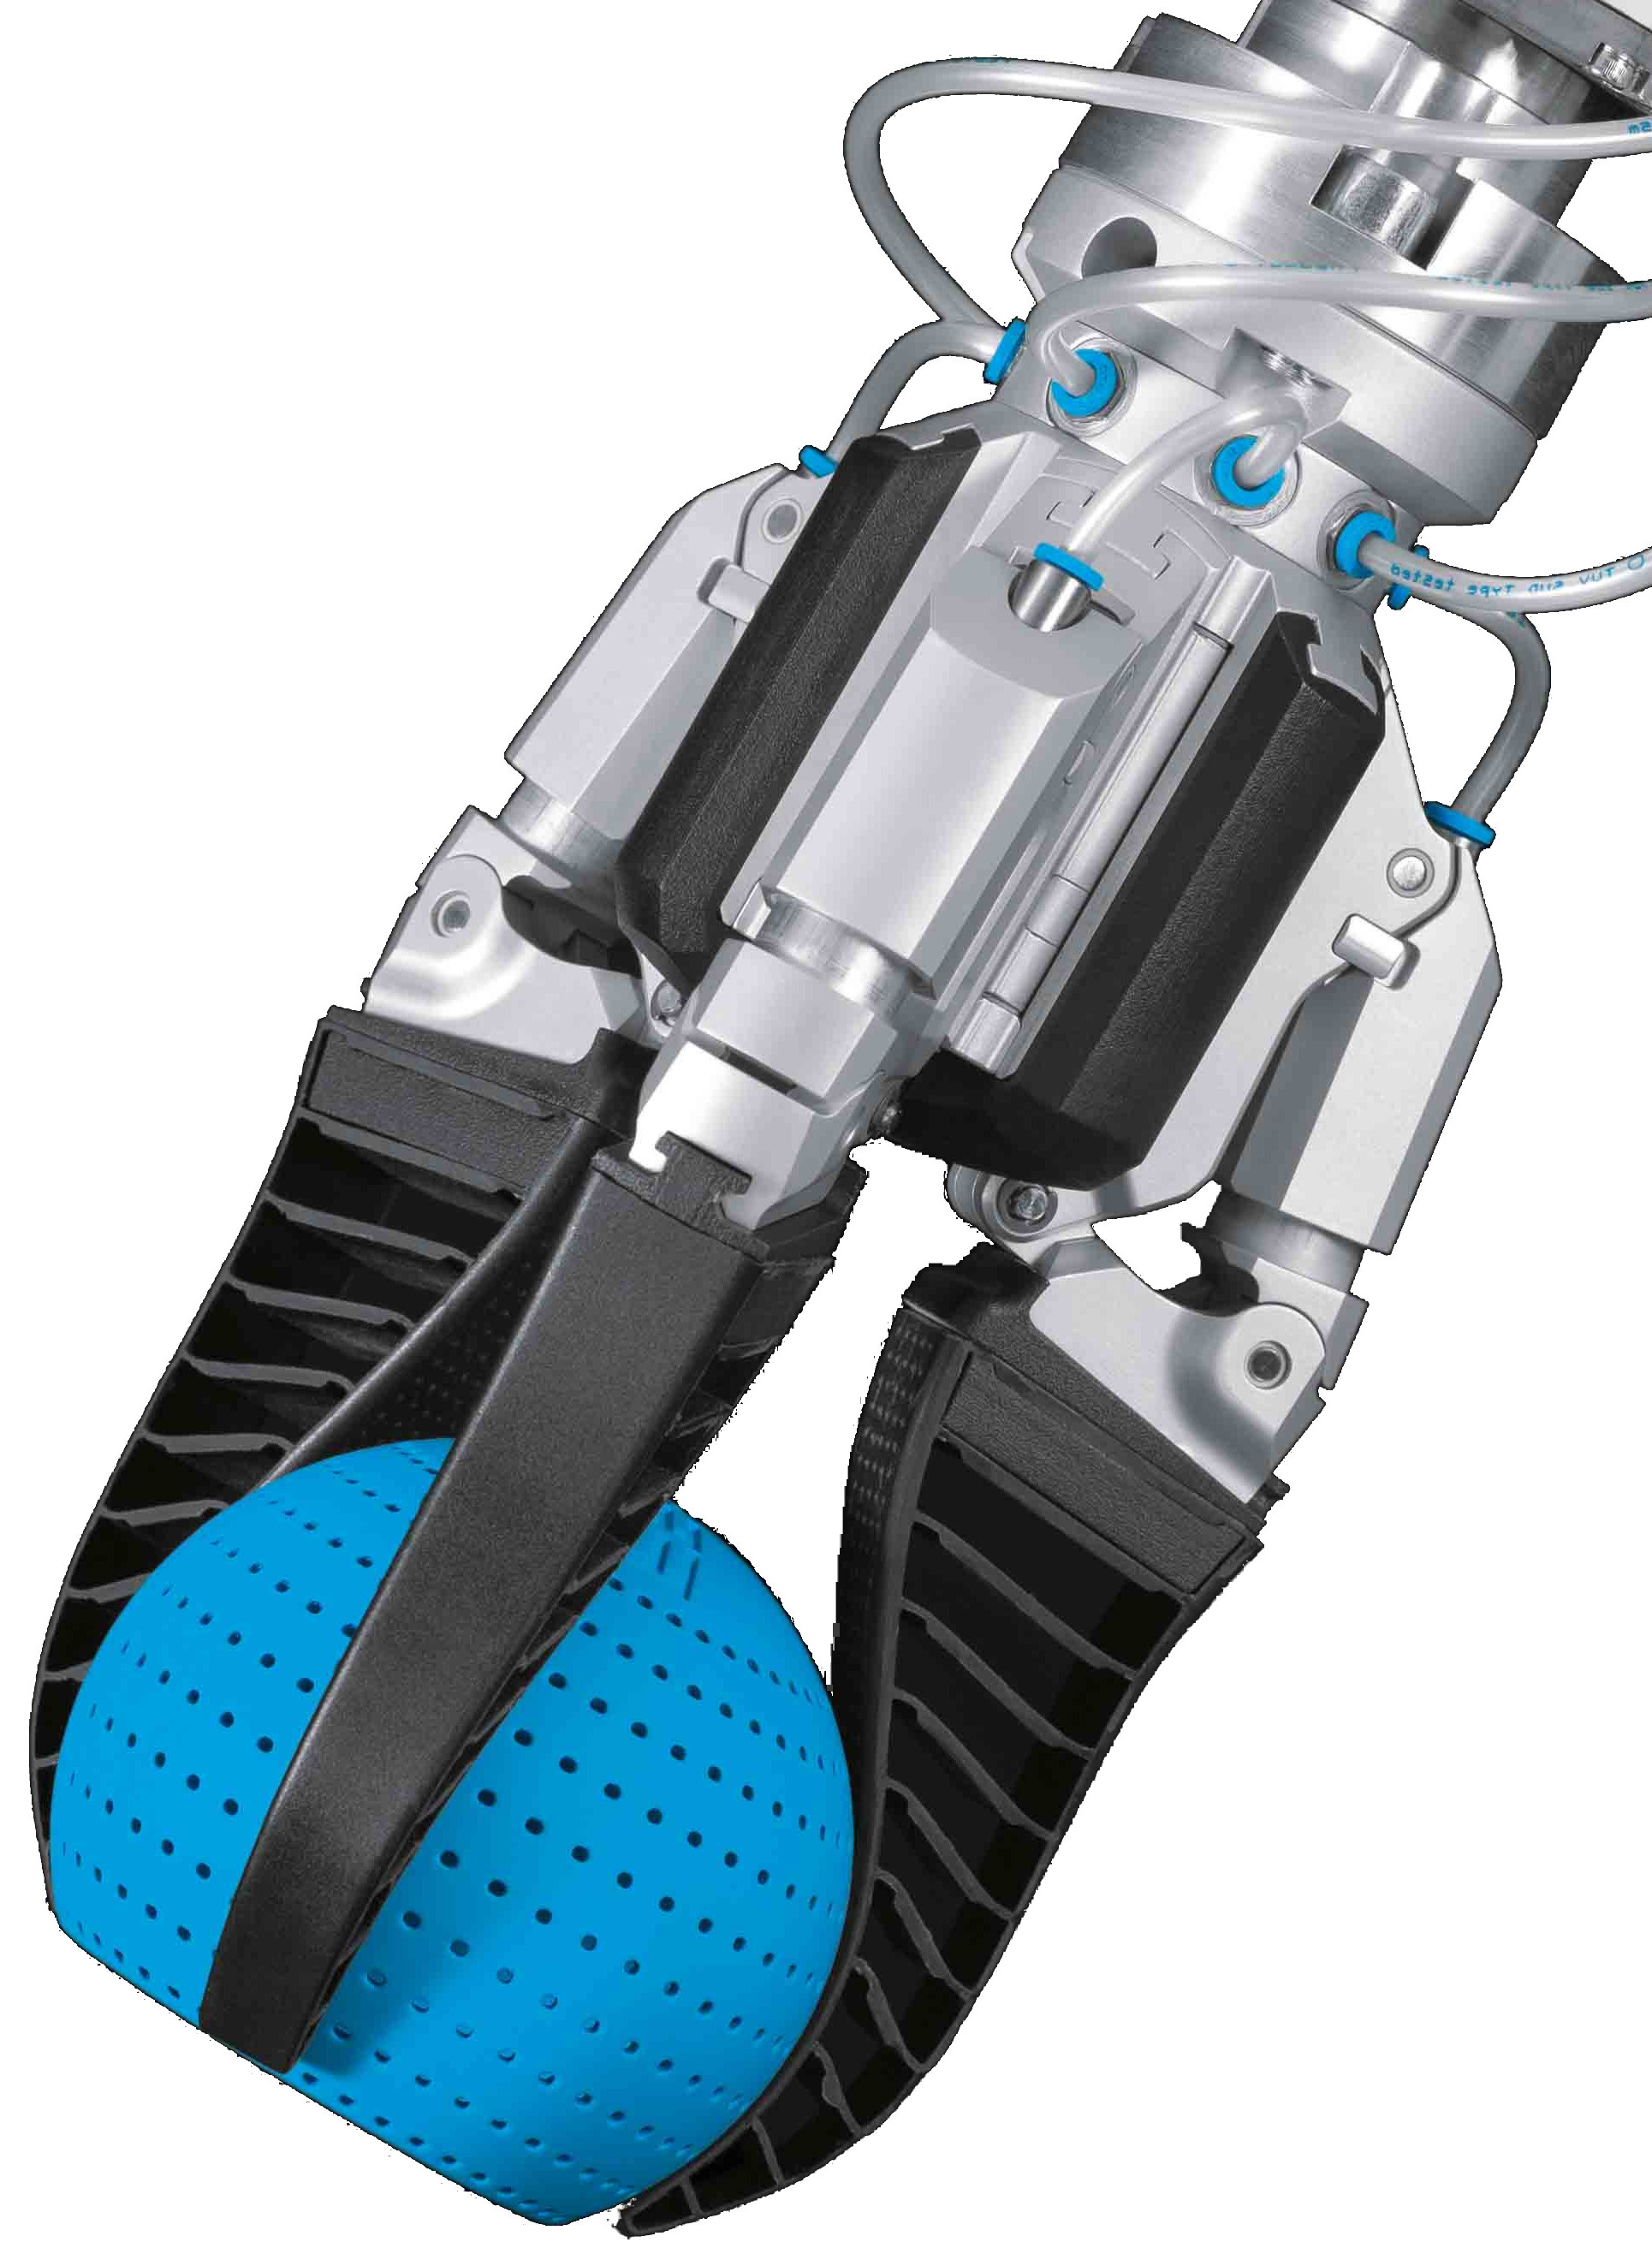
\includegraphics[height=.17\textheight]{grippers/festo-multichoice-gripper}}
		{\caption[Festo flexible 3 finger gripper]{Festo flexible 3 finger gripper\protect\footnotemark}\label{fig:festo-multichoice-gripper}}

		\ffigbox[1\FBwidth]
		{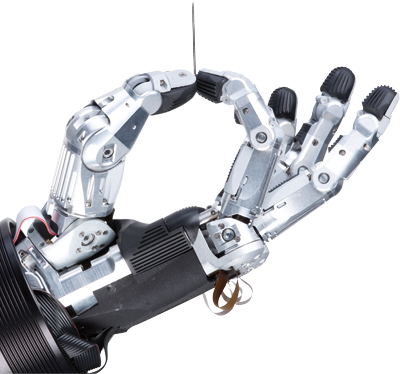
\includegraphics[height=.17\textheight]{grippers/schunk-svh-precision-grip}}
		{\caption[Schunk anthropomorphic gripper]{Schunk anthropomorphic gripper\protect\footnotemark}\label{fig:schunk-svh-hand}}
	\end{floatrow}
\end{figure}
\footnotetext[\the\numexpr\value{footnote}-3\relax]{\url{http://blog.robotiq.com/topic/2-finger-robot-gripper}}
\footnotetext[\the\numexpr\value{footnote}-2\relax]{\url{http://support.robotiq.com/display/IMB/Home}}
\footnotetext[\the\numexpr\value{footnote}-1\relax]{\url{https://www.festo.com/group/en/cms/10221.htm}}
\footnotetext[\value{footnote}]{\url{http://mobile.schunk-microsite.com/en/produkte/products/servo-electric-5-finger-gripping-hand-svh.html}}


\begin{figure}[H]
	\begin{floatrow}[4]
		\ffigbox[2.4\FBwidth]
		{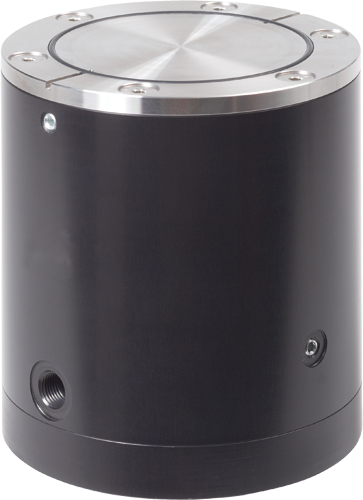
\includegraphics[height=.08\textheight]{grippers/zimmer-magnetic-gripper}}
		{\caption[Zimmer magnetic gripper]{Zimmer magnetic gripper\protect\footnotemark}\label{fig:zimmer-magnetic-gripper}}

		\ffigbox[1.98\FBwidth]
		{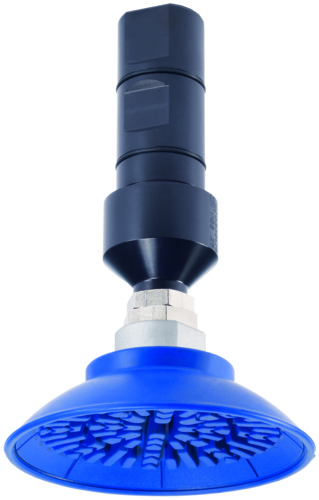
\includegraphics[height=.11\textheight]{grippers/schunk-vacuum-gripper}}
		{\caption[Schunk vacuum gripper]{Schunk vacuum gripper\protect\footnotemark}\label{fig:schunk-vacuum-gripper}}

		\ffigbox[2\FBwidth]
		{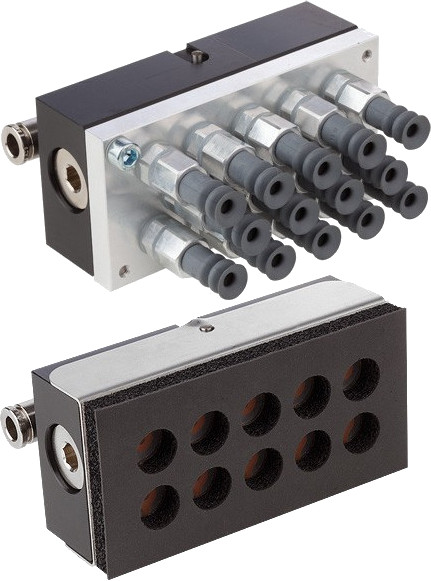
\includegraphics[height=.1\textheight]{grippers/schmalz-vacuum-area-gripper}}
		{\caption[Schmalz vacuum area gripper]{Schmalz vacuum area gripper\protect\footnotemark}\label{fig:schmalz-vacuum-area-gripper}}

		\ffigbox[\FBwidth]
		{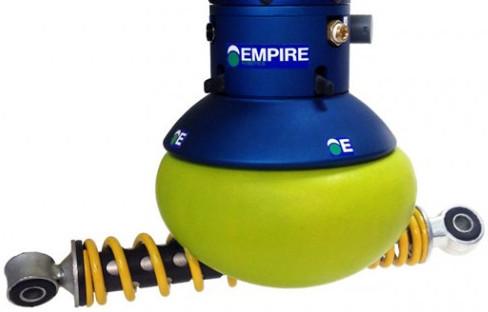
\includegraphics[height=.11\textheight]{grippers/versa-ball}}
		{\caption[Versa ball]{Versa ball\protect\footnotemark}\label{fig:versa-ball}}
	\end{floatrow}
\end{figure}
\footnotetext[\the\numexpr\value{footnote}-3\relax]{\url{http://www.zimmer-group.de/en/ajax/productdetail?struktkey=\%24MN-SOM-\%24PLC-V-\%24PG-GRE-\%24SR-HM1000&productkey=HM1097NC&layout=1}}
\footnotetext[\the\numexpr\value{footnote}-2\relax]{\url{http://de.schunk.com/de_en/gripping-systems/\#/series/gsw-v}}
\footnotetext[\the\numexpr\value{footnote}-1\relax]{\url{https://www.schmalz.com/en/vacuum-technology-for-automation/vacuum-components/area-gripping-systems-and-end-effectors}}
\footnotetext[\value{footnote}]{\url{http://www.extremetech.com/extreme/174723-soft-robotic-gripper-uses-vacuum-pressure-and-a-beanbag-to-move-objects}}

%Articles:\\
%- An overview of 3D object grasp synthesis algorithms
%- A review on importance of universal gripper in industrial robot applications
%- A survey of bio-inspired robotics hands implementation - New directions in dexterous manipulation

%Articles:\\
%- An Adaptive Feedback Scheduling Algorithm for Robot Assembly and Real-Time Control Systems


\subsection{Automatic tool change}

Given the wide variety of objects that assembly operations may require, automatic tool change devices (such as the one shown in \cref{fig:tool-changer}) are very useful to allow the robot to autonomously change the end effector in order to perform the current task with the most appropriate hardware configuration.

\begin{figure}[H]
	\centering
	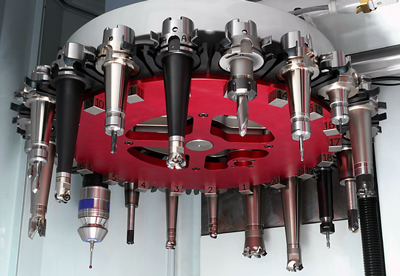
\includegraphics[width=0.66\linewidth]{grippers/tool-changer}
	\caption[Automatic tool changer with 20 different robotic arm end effectors]{Automatic tool changer with 20 different robotic arm end effectors\protect\footnotemark}
	\label{fig:tool-changer}
\end{figure}
\footnotetext{\url{http://www.h-h.com.au/ae_mc_tool-changer.htm}}


\subsection{Environment fixtures}

Environment fixtures are a very useful approach to ensure that the assembly objects are provided by the human operator at known positions with high accuracy (avoiding complex perception systems). These fixtures can be in the form of packaging trays (example in \cref{fig:vacuum-formed-packaging-trays}) allowing quick restock of assembly objects or can be inclined loading docks (example in \cref{fig:parts-loading-fixture}), in which the human operators insert the assembly objects at the top and robot removes them always at the same place at the bottom (when the robot removes one object the gravity pulls the next one into place).

Another useful application of environment fixtures is for temporarily holding the assembly objects, either using static fixtures (examples in \cref{fig:profile-vertical-fixture,fig:profile-horizontal-fixture}) or actuated grippers (example in \cref{fig:part-fixture-actuated}). This can be very useful to allow assembly operations with only one robotic arm and also for changing gripping positions of grasped objects (examples in \cref{fig:part-fixture-actuated} and \cite{Chavan2015}).

%Articles:\\
%- Prehensile Pushing - In-hand Manipulation with Push-Primitives | Chavan2015

\begin{figure}[H]
	\begin{floatrow}[2]
		\ffigbox[\FBwidth]
		{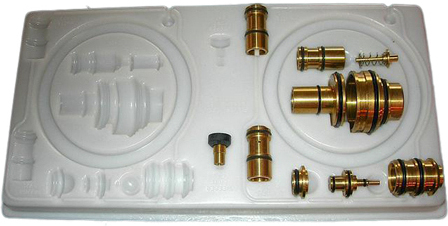
\includegraphics[height=.183\textheight]{grasping/vacuum-formed-packaging-trays}}
		{\caption[Vacuum formed packaging tray]{Vacuum formed packaging tray\protect\footnotemark}\label{fig:vacuum-formed-packaging-trays}}

		\ffigbox[\FBwidth]
		{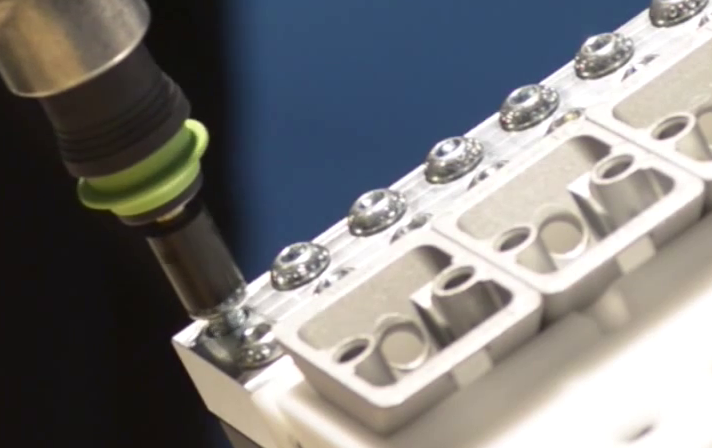
\includegraphics[height=.183\textheight]{grasping/parts-loading-fixture}}
		{\caption[Parts loading dock]{Parts loading dock\protect\footnotemark}\label{fig:parts-loading-fixture}}
	\end{floatrow}
\end{figure}
\footnotetext[\the\numexpr\value{footnote}-1\relax]{\url{http://www.vinayakapolyproducts.com/vacuum-formed-packaging-trays-2186055.html}}
\footnotetext[\value{footnote}]{\url{https://www.youtube.com/watch?v=2jYhdmk-pMg}}

\begin{figure}[H]
	\begin{floatrow}[3]
		\ffigbox[\FBwidth]
		{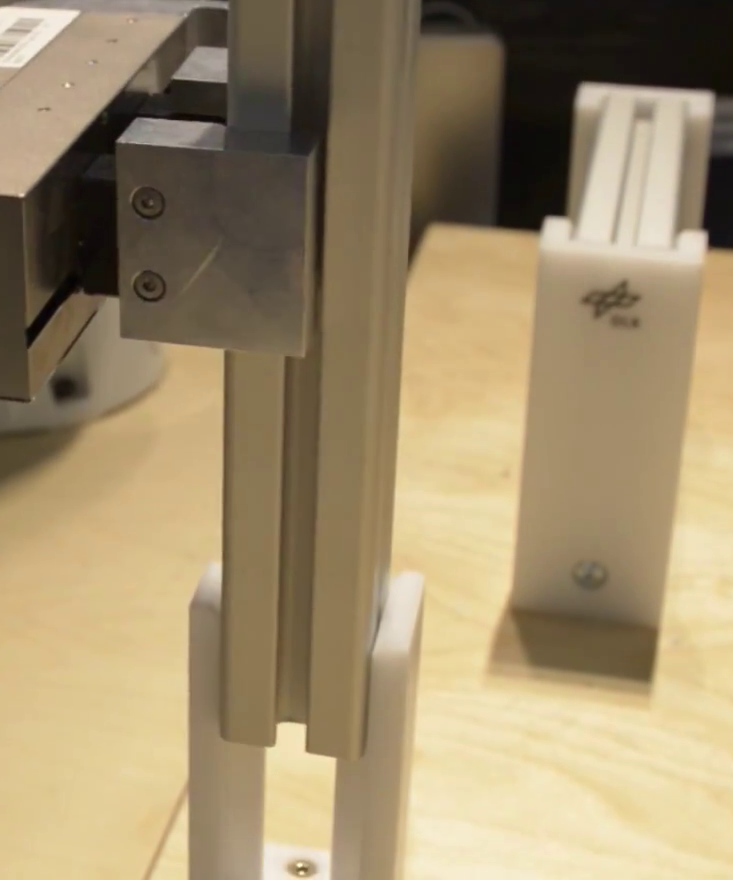
\includegraphics[height=.22\textheight]{grasping/profile-vertical-fixture}}
		{\caption[Aluminum profile vertical fixture]{Aluminum profile vertical fixture\protect\footnotemark[\value{footnote}]}\label{fig:profile-vertical-fixture}}

		\ffigbox[\FBwidth]
		{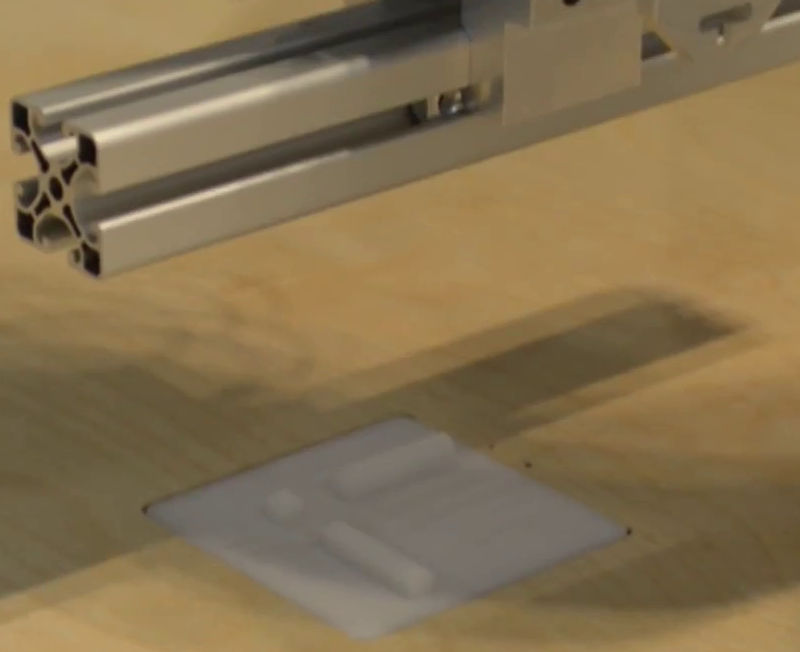
\includegraphics[height=.22\textheight]{grasping/profile-horizontal-fixture}}
		{\caption[Aluminum profile horizontal fixture]{Aluminum profile horizontal fixture\protect\footnotemark[\value{footnote}]}\label{fig:profile-horizontal-fixture}}

		\ffigbox[\FBwidth]
		{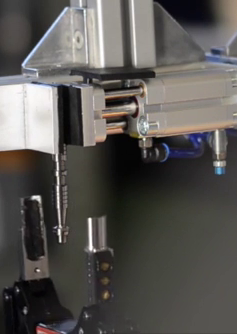
\includegraphics[height=.22\textheight]{grasping/part-fixture-actuated}}
		{\caption[Actuated object holder]{Actuated object holder\protect\footnotemark}\label{fig:part-fixture-actuated}}
	\end{floatrow}
\end{figure}
\footnotetext[\value{footnote}]{\url{https://www.youtube.com/watch?v=MuKOPnrYS-Q}}



\subsection{Alignment devices}

Assembling objects is a very complex task that requires accurate perception and pose estimation of the assembly parts and also proper gripping positioning. For interconnected objects, force-torque sensors and alignment devices such as \glspl{rcc} (example in \cref{fig:remote-center-compensator}) can be very useful tools for tolerating small misalignments and ensuring proper part installation.

\begin{figure}[H]
	\centering
	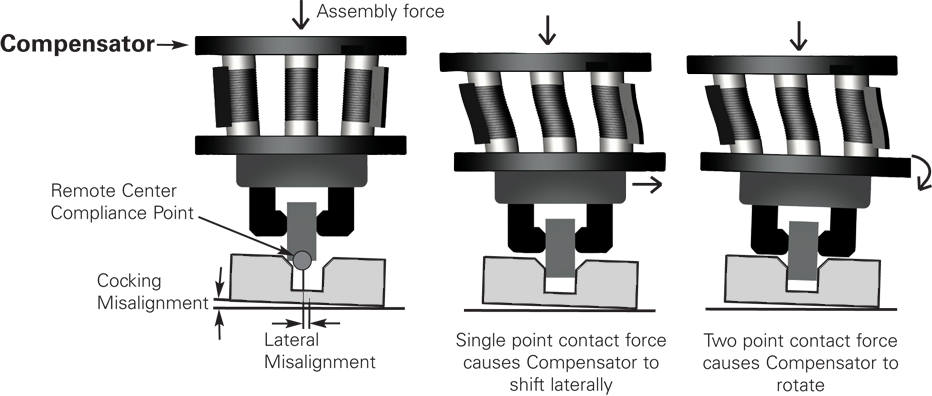
\includegraphics[width=0.88\linewidth]{grasping/remote-center-compensator}
	\caption[Usage of a \glsentrytext{rcc} to tolerate slight part misalignments]{Usage of a \glsentrytext{rcc} to tolerate slight part misalignments\protect\footnotemark}
	\label{fig:remote-center-compensator}
\end{figure}
\footnotetext{\url{http://www.ati-ia.com/products/compliance/Compensator_product_desc.aspx}}


\subsection{Motion planners}

Planning the coordinated motion of robotic arms and grippers in assembly operations requires advanced path planning algorithms \cite{Fontanals2014,You2012,mopl2015} and needs to take in consideration the robot hardware configuration and manipulation capabilities along with the world state and assembly knowledge \cite{Tenorth14} (such as where are the parts to be assembled and in which order they will be installed). This knowledge integration is critical in order to generate the assembly graph with the proper part installation sequence that ensures that the robot will be able to use its end effectors to perform all the tasks \cite{Thomas2003ATP,Thomas2011}.


%Articles:\\
%- A new probabilistic path planning algorithm for (dis) assembly tasks\\
%+ Development of Manipulation Planning Algorithm for a Dual-arm Robot Assembly Task\\ | You2012
%+ Integrated Grasp and Motion Planning using Independent Contact Regions\\ | Fontanals2014
%+ Knowledge-based Specification of Robot Motions\\ | Tenorth14
%- MOPL - A Multi-Modal Path Planner for Generic Manipulation Tasks
%- Assembly Planning and Task Planning - Two Prerequisites for Automated Robot Programming\\ | Thomas2011
%- Efficient assembly sequence planning using stereographical projections of c-space obstacles\\ | Thomas2003ATP



\section{Perception sensors}

Perception sensors for object recognition have evolved dramatically in the last few years, with the emergence of RGB-D and \gls{tof} sensors (such as the Kinect 1 and 2) as an affordable and reasonably accurate technological solution. Other perception sensors commonly used include 2D and stereo cameras and also camera-laser systems.


\subsection{Image acquisition}\label{sec:image-acquisition}

With the increase of resolution and lens build quality, 2D sensors remain a viable and accurate solution for detecting objects and perform quality inspection. Moreover, when used to observe the environment from several perspectives, they can achieve good geometry reconstruction and allow accurate 3D perception of objects. The two main image acquisition technologies (\gls{cmos} and \gls{ccd}) are shown in \cref{fig:ccd} and \cref{fig:cmos}.


\begin{figure}[H]
	\begin{floatrow}[2]
		\ffigbox[\FBwidth]
		{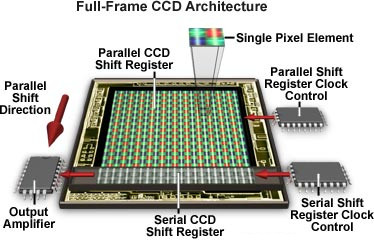
\includegraphics[height=.21\textheight]{sensors/ccd}}
		{\caption[\glsentrytext{ccd} sensor]{\glsentrytext{ccd} sensor\protect\footnotemark}\label{fig:ccd}}

		\ffigbox[\FBwidth]
		{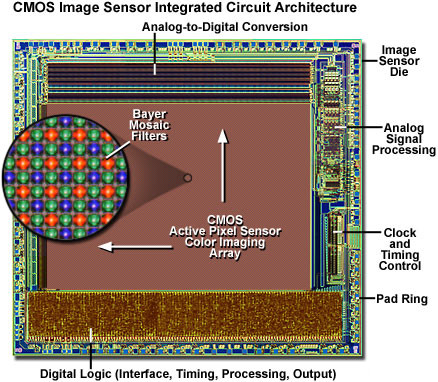
\includegraphics[height=.21\textheight]{sensors/cmos}}
		{\caption[\glsentrytext{cmos} sensor]{\glsentrytext{cmos} sensor\protect\footnotemark}\label{fig:cmos}}
	\end{floatrow}
\end{figure}
\footnotetext[\the\numexpr\value{footnote}-1\relax]{\url{http://cctvsystemblog.blogspot.pt/2013/07/architecture-of-ccd.html}}
\footnotetext[\value{footnote}]{\url{https://micro.magnet.fsu.edu/primer/digitalimaging/cmosimagesensors.html}}


\subsection{Point cloud acquisition}\label{sec:point-cloud-acquisition}

Point clouds can be retrieved with a wide range of sensors with varying levels of precision and acquisition time \cite{Sansoni2009}. The next sections provide a brief overview of the main technologies capable of generating accurate point clouds useful for 3D perception.


\subsubsection{Camera-laser systems}

Camera-laser systems can obtain 3D geometry information from the environment by analyzing the deformation pattern of the laser light that is projected into the scene at incremental positions (example in \cref{fig:laser-triangulation}). They can achieve very accurate results, but given the need to physically move the laser or the object to scan, they require longer acquisition periods than the methods presented below.

\begin{figure}[H]
	\centering
	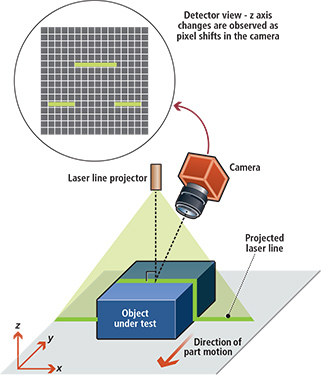
\includegraphics[width=0.4\linewidth]{sensors/laser-triangulation}
	\caption[Camera laser 3D triangulation system]{Camera laser 3D triangulation system\protect\footnotemark}
	\label{fig:laser-triangulation}
\end{figure}
\footnotetext{\url{http://www.vision-systems.com/articles/print/volume-20/issue-6/features/understanding-laser-based-3d-triangulation-methods.html}}


\subsubsection{Stereo vision methods}

Stereo vision systems (example in \cref{fig:stereo-cameras}) can generate 3D representations of the environment by comparing the displacement of corresponding points in the two ambient images (\cref{fig:stereo-vision} gives an overview of such a system). This can be achieved because the relative position of the cameras is known. As such, points farther away will have smaller displacement between images than points closer to the cameras. In the end, a disparity image is obtained, that can then be converted to a point cloud representation of the environment.

Given that the accuracy of the disparity image relies heavily in the correct matching of points between the left and right image, some stereo vision systems employ active observation by projecting a pattern into the environment in order to refine the point matching (example of hardware setup in \cref{fig:pr2-active-stereo}). This can significantly improve the accuracy if the environment has a lot of smooth surfaces with homogeneous colors.

\begin{figure}[H]
	\begin{floatrow}[2]
		\ffigbox[\FBwidth]
		{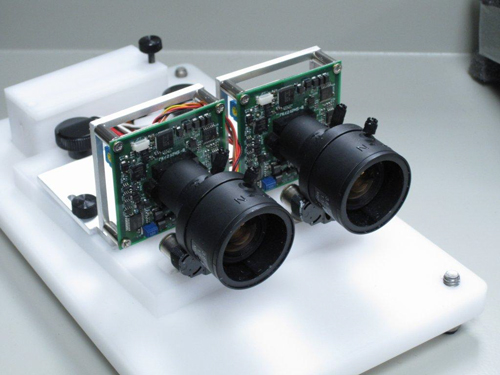
\includegraphics[height=.15\textheight]{sensors/stereo-cameras}}
		{\caption[Stereo vision system]{Stereo vision system \cite{Kaczurba2013}}\label{fig:stereo-cameras}}

		\ffigbox[\FBwidth]
		{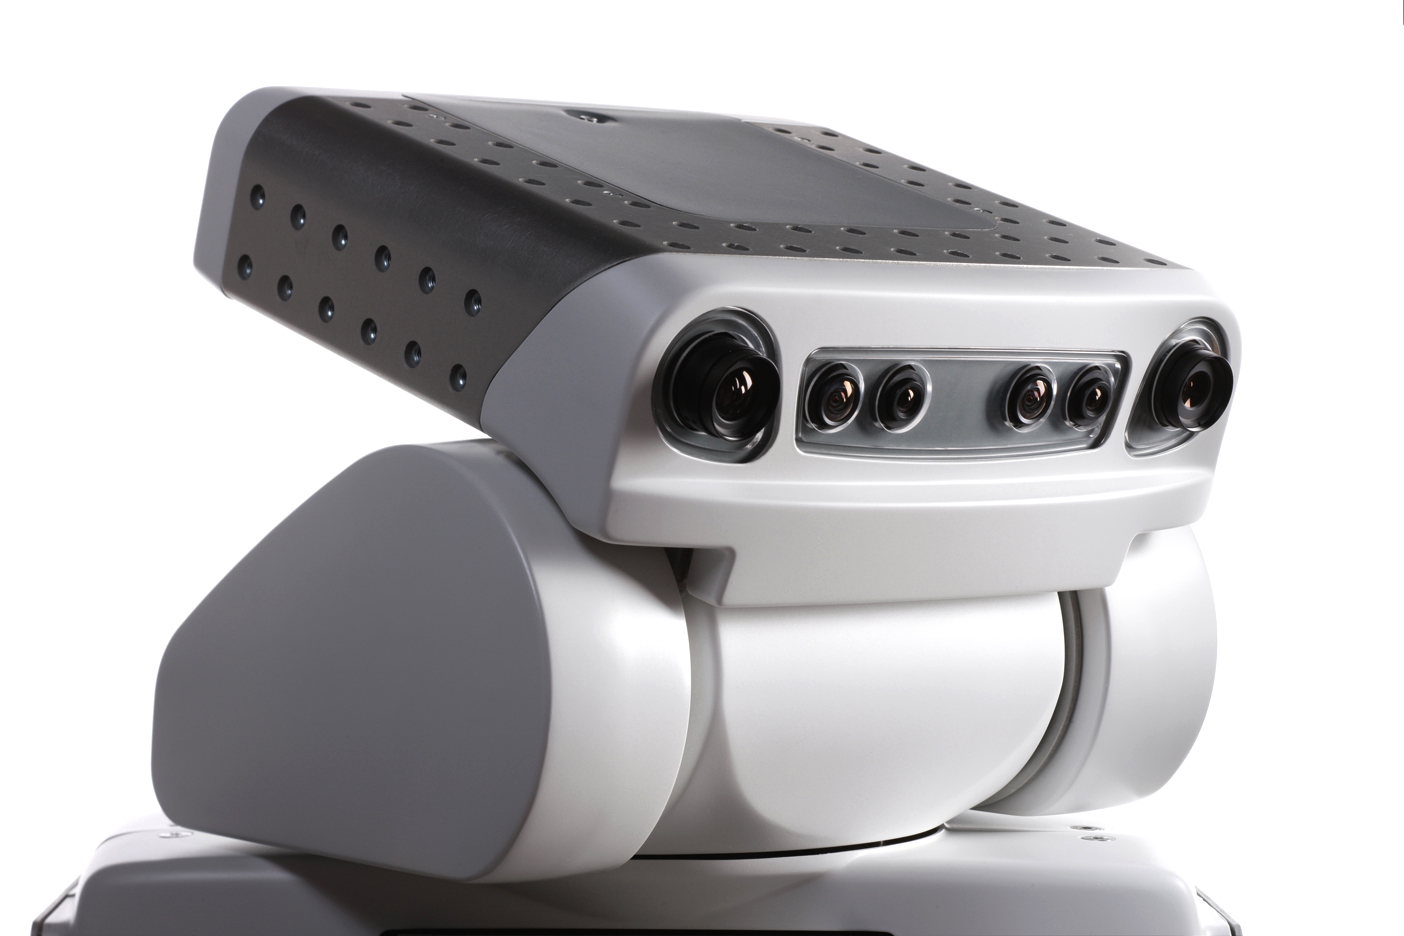
\includegraphics[height=.15\textheight]{sensors/pr2-active-stereo}}
		{\caption[PR2 head capable of active stereo vision]{PR2 head capable of active stereo vision\protect\footnotemark}\label{fig:pr2-active-stereo}}
	\end{floatrow}
\end{figure}
\footnotetext{\url{https://www.willowgarage.com/pages/pr2/overview}}


\begin{figure}[H]
	\centering
	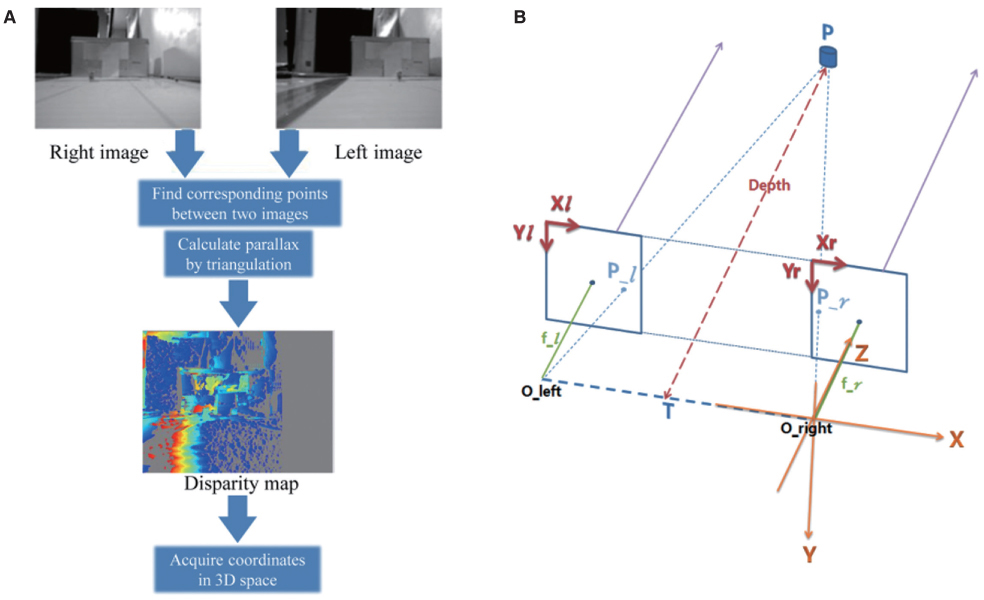
\includegraphics[height=.33\textheight]{sensors/stereo-vision}
	\caption[Stereo vision overview]{Stereo vision overview \cite{Yang2014}}
	\label{fig:stereo-vision}
\end{figure}


\subsubsection{Structured light methods}

Structured light methods can retrieve 3D geometry from images by projecting a known pattern into the environment and analyzing its deformation (examples in \Cref{fig:structured-light,fig:kinect1-ir}). They can achieve sample rates of 30 Hz and besides 3D geometry they can also retrieve color information.


\begin{figure}[H]
	\begin{floatrow}[2]
		\ffigbox[\FBwidth]
		{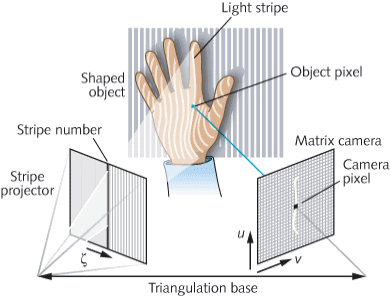
\includegraphics[height=.21\textheight]{sensors/structured-light}}
		{\caption[Structured light system diagram]{Structured light system diagram\protect\footnotemark}\label{fig:structured-light}}

		\ffigbox[\FBwidth]
		{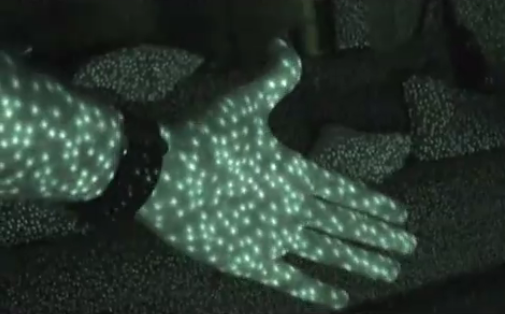
\includegraphics[height=.21\textheight]{sensors/kinect1-ir}}
		{\caption[Kinect 1 \glsentrytext{ir} pattern]{Kinect 1 \glsentrytext{ir} pattern\protect\footnotemark}\label{fig:kinect1-ir}}
	\end{floatrow}
\end{figure}
\footnotetext[\the\numexpr\value{footnote}-1\relax]{\url{http://www.laserfocusworld.com/articles/2011/01/lasers-bring-gesture-recognition-to-the-home.html}}
\footnotetext[\value{footnote}]{\url{https://jahya.net/blog/how-depth-sensor-works-in-5-minutes}}


The Kinect sensor seen in \cref{fig:kinect1} is an example of a structured light system that can achieve measurements with millimeter accuracy for objects close to the sensor. Another similar sensor is the Occipital Structure IO\footnote{\url{http://structure.io/}} which is intended for mobile devices and can be seen in \cref{fig:structure-io}.


\begin{figure}[H]
	\begin{floatrow}[2]
		\ffigbox[1.1\FBwidth]
		{\includegraphics[height=.15\textheight]{sensors/kinect1}}
		{\caption[Kinect 2 sensor]{Kinect sensor\protect\footnotemark}\label{fig:kinect1}}

		\ffigbox[\FBwidth]
		{\includegraphics[height=.15\textheight]{sensors/structure-io}}
		{\caption[Structure IO sensor]{Structure IO sensor\protect\footnotemark}\label{fig:structure-io}}
	\end{floatrow}
\end{figure}
\footnotetext[\the\numexpr\value{footnote}-1\relax]{\url{https://msdn.microsoft.com/en-us/library/jj131033.aspx}}
\footnotetext[\value{footnote}]{\url{http://structure.io/press}}


\subsubsection{\glsentrydesc{tof} methods}\label{sec:tof-methods}

\gls{tof} or \gls{toa} methods can be used to calculate distances based on the amount of time that a given wave takes from the moment it is created to the moment it is received (system operation overview in \cref{fig:time-of-flight}). By acquiring a large amount of sensor readings, a 3D representation of the environment can be achieved.

Since these systems rely on active interaction with the environment, they can be used without being significantly affected by lighting interferences. Nevertheless, it should be taken in consideration the conditions in which the waves propagate and also the geometry of the environment, because it can affect the path that the waves take, and as a result, lead to the decrease of precision in the measurements.


\paragraph{\glsentrytext{tof} cameras}

\gls{tof} cameras (examples in \cref{fig:mesa-sr4000,fig:kinect2}) can acquire 3D measurements of the environment with very high frame rate (30 Hz or even higher) allowing perception and mapping of the environment with very low latency, which can be a critical requirement in perception tasks that must react very fast to changes in their surroundings.

\begin{figure}[H]
	\centering
	\includegraphics[width=0.6\linewidth]{sensors/time-of-flight}
	\caption[\glsentrydesc{tof} system diagram]{\glsentrydesc{tof} system diagram\protect\footnotemark}
	\label{fig:time-of-flight}
\end{figure}
\footnotetext{\url{http://www.laserfocusworld.com/articles/2011/01/lasers-bring-gesture-recognition-to-the-home.html}}

\begin{figure}[H]
	\begin{floatrow}[2]
		\ffigbox[1.05\FBwidth]
		{\includegraphics[height=.16\textheight]{sensors/mesa-sr4000}}
		{\caption[Mesa SR4000 sensor]{Mesa SR4000 sensor\protect\footnotemark}\label{fig:mesa-sr4000}}

		\ffigbox[1.05\FBwidth]
		{\includegraphics[height=.16\textheight]{sensors/kinect2}}
		{\caption[Kinect 2 sensor]{Kinect 2 sensor\protect\footnotemark}\label{fig:kinect2}}
	\end{floatrow}
\end{figure}
\footnotetext[\the\numexpr\value{footnote}-1\relax]{\url{http://www.mesa-imaging.ch/products/product-overview}}
\footnotetext[\value{footnote}]{\url{https://www.ifixit.com/Teardown/Xbox+One+Kinect+Teardown/19725}}


\paragraph{\glsentrytext{lidar}}

Light waves generated with lasers can estimate distances with millimeter accuracy at long ranges and their sensors usually have a low sample rate (below 20 Hz). Systems like \gls{lidar} (3D sensor example shown in \cref{fig:velodyne-hdl-64e}) take advantage of this fact and can be used to obtain a very detailed 3D point cloud of the environment (like the one showed in \cref{fig:lidar-scan}). Moreover, some \glspl{lidar} can also capture the environment reflectivity / intensity besides their 3D geometry.

\begin{figure}[H]
	\begin{floatrow}[2]
		\ffigbox[]
		{\includegraphics[height=.14\textheight]{sensors/velodyne-hdl-64e}}
		{\caption[3D Velodyne HDL-64E]{3D Velodyne HDL-64E\protect\footnotemark}\label{fig:velodyne-hdl-64e}}

		\ffigbox[\FBwidth]
		{\includegraphics[height=.14\textheight]{sensors/lidar-scan-car}}
		{\caption[\glsentrytext{lidar} scan]{\glsentrytext{lidar} scan\protect\footnotemark}\label{fig:lidar-scan}}
	\end{floatrow}
\end{figure}
\footnotetext[\the\numexpr\value{footnote}-1\relax]{\url{http://www.velodynelidar.com/lidar/hdlproducts/hdl64e.aspx}}
\footnotetext[\value{footnote}]{\url{http://www.popsci.com/cars/article/2013-09/google-self-driving-car}}


\section{Perception systems}

There is a wide range of perception algorithms and sensors that can perform object recognition and pose estimation, either using 2D images \cite{Marton2011,Costa2016ICARSC} or 3D data \cite{Wohlkinger2012,Aldoma2011}. For very specific recognition tasks, template matching techniques \cite{Lee2016} or color / shape segmentation methods (such as simple \gls{hsv} thresholding, advanced segmentation using the watershed algorithm or fitting specific shapes to the sensor data using \gls{ransac} or the Hough transform \cite{Ballard1981}) provide a simple and effective approach. For more generic perception tasks, it is usually necessary to rely on feature detection \cite{Tuytelaars2008,Filipe2014} to select reliable keypoints, feature description \cite{Gauglitz2011,Hansch2014} to characterize the geometry around each interest point and robust matching algorithms (for example \gls{ransac} coupled with \gls{knn} descriptor association and \gls{svd} pose estimation) in order to be able to recognize the objects even in cluttered environments \cite{Aldoma2016}. Other approaches rely on machine learning classifiers \cite{Rocha2015} (such as \glspl{svm}, \glspl{nn}, \glspl{dt}, \glspl{hmm}) and bag of words methods \cite{Csurka04,Costa2014,Nowak2006} in order to detect class of objects that have similar geometry and may appear in different perspectives. After the recognition stage, tracking algorithms such as Kalman \cite{Kalman1960} / particle filters \cite{Cho2006} coupled with accurate matching algorithms (for example MeanShift / CamShift \cite{Bradski1998} / \gls{icp} \cite{Besl1992}) can be used to follow the objects pose with high precision over time.

Some preliminary work has already been done in the area of 2D / 3D perception. In \cref{fig:banknote-recognition} it is shown a 2D perception system for detecting planar objects in which it is highlighted the typical processing steps required along with the most common algorithms used to estimate the 3D pose of objects from 2D images. In \cref{fig:localization-system} it is shown a similar 3D perception system that is able to perform 3D pose estimation of an object / robot from 3D sensor data.


%Articles:\\
%+ Combined 2D-3D Categorization and Classification for Multimodal Perception Systems | Marton2011
%
%Articles 2d:\\
%+ Evaluation of Interest Point Detectors and Feature Descriptors for Visual Tracking\\
%- Evaluation of interest point detectors for image information extraction\\
%- Local Invariant Feature Detectors - A Survey
%- Object Recognition from Local Scale-Invariant Features
%
%Articles 3d:\\
%+ 3DNet - Large-Scale Object Class Recognition from CAD Models\\ | Wohlkinger2012
%- 3D Visual Perception System for Bin Picking in Automotive Sub-Assembly Automation\\
%+ CAD-Model Recognition and 6DOF Pose Estimation Using 3D Cues\\ | Aldoma
%- Detecting and Segmenting Objects for Mobile Manipulation\\
%- Development of a 3D model based part recognition system for industrial applications - Main challenges\\ | Rocha2015
%+ A Global Hypothesis Verification Framework for 3D Object Recognition in Clutter
%- Scene Perception and Recognition in Industrial Environments for Human-Robot Interaction


\clearpage

\begin{figure}[H]
	\centering
	\begin{minipage}[h]{.54\textwidth}
		\centering
		\includegraphics[width=\linewidth]{banknote-recognition/system-overview}
	\end{minipage}%
	\begin{minipage}[h]{.26\textwidth}
		\centering
		\vspace*{.37em}
		\includegraphics[width=.485\linewidth]{banknote-recognition/notes-masks/500eu-front}
		\includegraphics[width=.485\linewidth]{banknote-recognition/notes-masks/500eu-front-mask}
		
		\vspace*{0.8em}
		\includegraphics[width=.485\textwidth]{banknote-recognition/preprocessing/500-500-500}
		\includegraphics[width=.485\textwidth]{banknote-recognition/preprocessing/500-500-500-preprocessed}
		
		\vspace*{1.2em}
		\includegraphics[width=.2496\textwidth]{banknote-recognition/image-resolution/500eu-front-very-low}\hfill
		\includegraphics[width=.2496\textwidth]{banknote-recognition/image-resolution/500eu_front_currencyDB_veryLowResolution_SIFT-Detector}\hfill
		\includegraphics[width=.2499\textwidth]{banknote-recognition/image-resolution/500eu-front-medium}\hfill
		\includegraphics[width=.2499\textwidth]{banknote-recognition/image-resolution/500eu_front_currencyDB_mediumResolution_SIFT-Detector}
		
		\vspace*{.9em}
		\includegraphics[width=.99\textwidth]{banknote-recognition/notes-recognition/5__(5).jpg___SIFT-Detector_SIFT-Extractor_BF-Matcher_lowQualityImageDB_globalMatch__inliersMatches__0}
		\includegraphics[width=.8\textwidth]{banknote-recognition/notes-recognition/20__(13).jpg___SIFT-Detector_SIFT-Extractor_BF-Matcher_mediumQualityImageDB_globalMatch__inliersMatches__0}
		
		\vspace*{.8em}
		\includegraphics[width=0.75\textwidth]{banknote-recognition/notes-masks/currency-db-shapes}
		
		\vspace*{.5em}
		\includegraphics[width=0.8\textwidth]{banknote-recognition/notes-recognition/10-20-50.jpg___SIFT-Detector_SIFT-Extractor_BF-Matcher_dynamicQualityImageDB_globalMatch}
	\end{minipage}
	\caption[Overview of a 2D perception system for planar object recognition]{Overview of a 2D perception system for planar object recognition \cite{Costa2016ICARSC}}
	\label{fig:banknote-recognition}
\end{figure}

\begin{figure}[H]
	\centering
	\includegraphics[height=.41\textheight]{self-localization/localization-system-modules}
	\includegraphics[height=.41\textheight]{self-localization/localization-system-overview}
	\caption[Overview of a 3D perception system for object / robot pose estimation]{Overview of a 3D perception system for object / robot pose estimation \cite{Costa2016Elsevier}}
	\label{fig:localization-system}
\end{figure}



\section{Knowledge management}

Creation and management of reusable knowledge across robots with different hardware configurations is a challenging task that can be solved by using cloud robotics coupled with ontology databases and skill frameworks. The next sections present a brief overview of the application of these approaches to robotic assembly systems.


\subsection{Ontologies}

Ontologies allow to model world information in a structured and object oriented approach \cite{Stenmark2015}, which can be useful to store information about the assembly objects \cite{Perzylo2015}, such as its \gls{cad} data, their spatial disposition and other meta-information relevant for the assembly process (for example the torque or direction required to insure proper objects coupling).

%Articles:\\
%+ An ontology for CAD data and geometric constraints as a link between product models and semantic robot task descriptions | Perzylo2015
%+ Knowledge-based instruction of manipulation tasks for industrial robotics | Stenmark2015


\subsection{Skills}

Automation of assembly operations in industrial applications \cite{Patel2012} is a multi-disciplinary challenging task that orchestrates and manages the assembly operation graph and requires the integration of the robot motion planners with the gripping tools \cite{Thomas2015} along with the perception systems. Moreover, these assembly operations need to be reusable \cite{Butting2016,Andersen2014} between robots with different hardware configurations \cite{Thomas2002} but with equivalent assembly capabilities. This can be achieved by modeling assembly operations as abstract skills \cite{Holz2015} that can be executed with fault tolerance \cite{ThomasICRA2003} on top of a primitive software layer that models reusable operations, which in turn are executed on top of a device layer that transforms the abstract knowledge into robot perception and motion commands (diagram of skill based assembly system in \cref{fig:skiros}). These skills can either be automatically extracted from \gls{cad} / \gls{sop} analysis \cite{Thomas2001} or using a high level language, such as \gls{uml} \cite{ThomasICRA2013}.

\begin{figure}[H]
	\centering
	\includegraphics[width=0.5\linewidth]{related-work/skiros}
	\caption[Skill-based Architecture SkiROS]{Skill-based Architecture SkiROS \cite{Holz2015}}
	\label{fig:skiros}
\end{figure}


%Articles:\\
%+ A new skill based robot programming language using uml-p statecharts\\
%+ A system for automatic planning, evaluation and execution of assembly sequences for industrial robots\\
%- A unified notation for serial, parallel, and hybrid kinematic structures
%+ Enabling robots in small-part assembly lines\\
%+ Flexible assembly through integrated assembly sequence planning and grasp planning\\
%+ Modeling Reusable, Platform-Independent Robot Assembly Processes
%- A new framework for task oriented sensor based robot programming and verification\\
%+ A Skill-Based System for Object Perception and Manipulation for Automating Kitting Tasks\\
%+ Definition of Hardware-Independent Robot Skills for Industrial Robotic Co-workers\\
%+ Error-tolerant execution of complex robot tasks based on skill primitives\\
%- Skills for Vision-based Applications in Robotics Application to aeronautics assembly pilot station


\subsection{Cloud robotics}

Given the reusable nature of assembly operations, cloud robotics can provide a communication and storage architecture for the distribution of new learned skills across a fleet of robots \cite{Tenorth2013} and could also allow to offload heavy computations, such as data mining \cite{Witten2005} and cognition related tasks \cite{Beetz2010,Tenorth2013k,Saxena2014,Beetz2015} from the robots embedded systems into more powerful processing servers \cite{Hunziker2013}.

%Articles:\\
%- On Distributed Knowledge Bases for Robotized Small-Batch Assembly\\
%+ KnowRob - A Knowledge Processing Infrastructure for cognition-enabled robots\\ | Tenorth2013
%+ OPEN-EASE - A Knowledge Processing Service for Robots and Robotics - AI Researchers\\ | Beetz2015
%+ Representation and exchange of knowledge about actions, objects, and environments in the roboearth framework\\ | Tenorth2013
%+ RoboBrain - Large-Scale Knwoledge Engine for Robots\\ | Saxena2014
%+ CRAM - A Cognitive Robot Abstract Machine for Everyday Manipulation in Human Environments\\ | Beetz2010
%+ Rapyuta - The RoboEarth Cloud Engine | Hunziker2013
%+ Data Mining - Practical Machine Learning Tools and Techniques (3rd Ed) | Witten2005



\section{Teaching systems}

There are several approaches to teaching new skills to robots ranging from advanced teach pendent / lead through programming, to the easy and intuitive usage of task level and \gls{cad} based specifications using tactile interfaces \cite{Perzylo2015a}. However, the teaching can be faster and more intuitive if the robot manages to learn new assembly knowledge \cite{tensorflow} by human demonstration \cite{Argall2009,Hamabe2015,Wang2015} using machine learning algorithms, such as those shown in \cref{fig:machinelearningalgorithms}.

\begin{figure}[H]
	\centering
	\includegraphics[width=\linewidth]{related-work/machinelearningalgorithms}
	\caption[Machine learning algorithms mind map]{Machine learning algorithms mind map\protect\footnotemark}
	\label{fig:machinelearningalgorithms}
\end{figure}
\footnotetext{\url{https://jixta.wordpress.com/2015/07/17/machine-learning-algorithms-mindmap}}

%Articles:\\
%- Efficient Model Learning from Joint-Action Demonstrations for Human-Robot Collaborative Tasks
%- Robust control of force-coupled human–robot-interaction in assembly processes\\
%+ Toward Efficient Robot Teach-In and Semantic Process Descriptions for Small Lot Sizes | Perzylo2015a
%+ TensorFlow - Large-Scale Machine Learning on Heterogeneous Distributed Systems | tensorflow
%+ A Programming by Demonstration System for Human-Robot Collaborative Assembly Tasks
%+ Multi-class Assembly Parts Recognition using Composite Feature and Random Forest for Robot Programming by Demonstration



\section{Human Machine Interaction systems}

There is a wide range of technologies that allow the exchange of information between humans and machines \cite{Goodrich2008}, from the typical display devices (screens, projectors) to natural interaction using visual and audio \cite{Yan2014} communication protocols. The next sections provide a brief overview of the human machine interaction systems that are useful for cooperative assembly operations.

%Articles:\\
%- A Survey on Perception Methods for Human-Robot Interaction in Social Robots\\ | Yan2014
%- Human-Robot Interaction - A Survey | Goodrich2008


\subsection{Augmented reality}

\gls{ar} interfaces offer an immersive way of exchanging information between a human operator and a machine \cite{Bimber2005}. One example of \gls{ar} systems is projection mapping \cite{Tan2013,Fujimoto2014} for environment marking of information, which is useful to indicate which object the operator should pick up next and where it should place it for assembly / welding / cutting operations (example in \cref{fig:laser-projection}). These systems allow accurate part positioning and avoid manual measurements by the human operator.

\begin{figure}[H]
	\centering
	\includegraphics[width=0.4\linewidth]{related-work/laser-projection}
	\caption[Projection mapping of cutting information]{Projection mapping of cutting information\protect\footnotemark}
	\label{fig:laser-projection}
\end{figure}
\footnotetext{\url{http://www.3dgage.com/laserprojection.html}}

%Articles:\\
%- Intuitive Robot Tasks with Augmented Reality and Virtual Obstacles\\
%+ iSarProjection - A KinectFusion Based Handheld Dynamic Spatial Augmented Reality System\\ | Tan2013
%+ Spatial Augmented Reality Merging Real and VirtualWorlds\\ | Bimber2005
%+ The Office of the Future - A Unified Approach to Image-Based Modeling and Spatially Immersive Displays | Raskar1998
%
%Articles projection mapping:\\
%- A Flexible Fringe Projection Vision System with Extended Mathematical Model for Accurate Three-Dimensional Measurement\\
%- Geometrically-Correct Projection-Based Texture Mapping onto a Deformable Object


\subsection{Natural language processing}

Natural language processing of unstructured textual representations can be very useful to extract assembly information from \glspl{sop} / operator manuals \cite{Stenmark2014,Stenmark2013} and speedup the robot leaning process \cite{Tenorth2010} (for example identifying which objects will be assembled, in which order and their approximate spatial distribution).

%Articles:\\
%- Connecting natural language to task demonstrations and low-level control of industrial robots\\
%- Describing constraint-based assembly tasks in unstructured natural language\\
%- Natural Language Programming of Industrial Robots\\
%- Understanding and Executing Instructions for Everyday Manipulation Tasks from the World Wide Web | Tenorth2010


\subsection{Human-robot cooperation}

Gesture recognition of operators hand movements \cite{Oikonomidis2012,Gleeson2013} is an important task when learning new assembly skills or when capturing new operator commands. Moreover, effective cooperation and exchange of information between humans and robots \cite{Putz2014} requires perception of the human body movements \cite{Roitberg2014} in order to recognize the operator intentions and detect when the robot should initiate or stop the interaction.


%Articles:\\
%- Analysis of Task-Based Gestures in Human-Robot Interaction\\
%+ Gestures for Industry - Intuitive Human-Robot Communication from Human Observation\\
%+ Human Activity Recognition in the Context of Industrial Human-Robot Interaction\\ | Roitberg2014
%- Human-Robot Communication for Collaborative Assembly
%
%Articles:\\
%- Coordination Mechanisms in Human-Robot Collaboration\\
%- Development of Collaborative Robots for Flexible Human Integrated Assembly Automation\\
%- Dynamic Emotion-Based Human-Robot Collaborative Assembly in Manufacturing\\
%- Human-Robot Collaborative Assembly by On-line Human Action Recognition Based on an FSM Task Model\\
%- Human-Robot Interaction for Cooperative Manipulation - Handing Objects to One Another\\
%- Identifying Nonverbal Cues for Automated Human-Robot Turn-taking\\
%- Information Support Development with Human-Centered Approach for Human-Robot Collaboration in Cellular Manufacturing



\section{Software frameworks}

Cooperative assembly of objects by robots is a multidisciplinary problem that requires advanced computer software systems. In order to speed up the implementation and deployment of the assembly system, several frameworks and libraries will be used. Among the most important are \gls{ros} for the system architecture, \gls{pcl} for the point cloud processing and Gazebo for simulation and testing.

\subsection{\glsentrytext{ros}}

\begin{wrapfigure}{r}{0.23\textwidth}
	\centering
	\vspace*{-2em}
	\includegraphics*[width=0.88\textwidth]{software/ros-logo}
	\caption{\glsentrytext{ros} logo}
	\label{fig:ros-logo}
\end{wrapfigure}

\gls{ros}\footnote{\url{http://www.ros.org}} \cite{Quigley2009} is a software framework designed to ease the development of robot systems. It provides seamless integration between hardware drivers and software modules, allowing a fast transition between simulation and deployment.

It's an open source project that offers a distributed computing framework with several core libraries and development tools that aims to speedup software prototyping, testing and deployment.


\subsubsection{Architecture}

The \gls{ros} architecture was designed from the beginning to be a distributed peer-to-peer software framework that could be deployed in several operating systems and implemented in a range of different programming languages. However, given that most of the \gls{ros} community prefers open source software, the Ubuntu\footnote{\url{http://www.ubuntu.com}} operating system is the main developing and testing environment, and as such, the recommended choice for \gls{ros} developers. Moreover, considering that robotics research requires software with both performance and maintainability at its core, the C++\footnote{\url{http://www.cplusplus.com}} programming language is used in most of the available packages, along with Python\footnote{\url{https://www.python.org}} and Java\footnote{\url{https://www.java.com}}.

Being a distributed computing framework, \gls{ros} relies in network connections and exchange of messages to perform the intended tasks. As such, its architecture was developed to follow a publish / subscribe pattern (\gls{ros} topics\footnote{\url{http://wiki.ros.org/Topics}}) and request and reply communication paradigm (\gls{ros} services\footnote{\url{http://wiki.ros.org/Services}} and actions\footnote{\url{http://wiki.ros.org/actionlib}}). This allows \gls{ros} nodes\footnote{\url{http://wiki.ros.org/Nodes}} (operating system processes) to be deployed in different computing platforms with ease and simplifies testing and exchange of software modules.

The next sections provide a more detailed description of the main \gls{ros} architecture concepts.


\paragraph{Nodes}

\gls{ros} nodes are operating system processes that are part of the peer-to-peer communication graph. They are the fundamental building blocks of any \gls{ros} system and can be spread among several computing platforms.

In order to manage the communications between nodes, the \gls{ros} framework provides a master node (roscore\footnote{\url{http://wiki.ros.org/roscore}}) that uses \gls{xmlrpc} to maintain a communication graph of the system. This allows nodes to be started without knowing the location (\gls{ip} address and port) of the other nodes in the network and greatly simplifies their integration and exchange. Also, by using \gls{ros} launch files\footnote{\url{http://wiki.ros.org/roslaunch}} (\gls{xml} configuration files), the specification of a system communication data flow and configuration can be easily altered.

Besides handling communications, the master node (roscore) also manages system configurations through the parameter server. This allows nodes to share and change the system configuration at runtime. However, given that the parameter server is usually queried only when a node starts up, the dynamic reconfigure\footnote{\url{http://wiki.ros.org/dynamic_reconfigure}} \gls{api} can be used instead, if it is necessary to change the configuration of a node when it is already running. This is achieved by providing a callback that is asynchronously called when a configuration change is requested.

The flexibility provided by \gls{ros} in both module integration and exchange can greatly speedup testing and deployment and the possibility of changing the configuration of the system at runtime and restart software modules individually (nodes) is very useful when implementing system supervisors and recovery behaviors.


\paragraph{Nodelets}

A nodelet\footnote{\url{http://wiki.ros.org/nodelet}} is a special kind of node that aims to reduce the overhead of message exchange. This overhead can be significant when messages are very large, such as point clouds or video. To mitigate this problem, the nodelets exchange pointers to shared memory regions, instead of sending the entire messages between nodes.

To achieve this overhead reduction, some architecture changes are required. The most important being the use of threads instead of processes, and the creation of a superclass that all nodelets must inherit. This leads to the creation of plugin libraries for each nodelet instead of an executable for each node.

Another important change is the introduction of nodelet managers to allow loading and setup of nodelets in different threads inside the same process.

In terms of implementation, the transition from nodes to nodelets requires few code changes and can lead to a significant improvement of the overall system performance.


\paragraph{Topics}

\gls{ros} topics are named communication buses that follow the publish / subscribe pattern. They provide a simple method for exchanging messages between nodes and allow the decoupling of information production and consumption. This is useful when there are multiple sources of the same information or there are multiple consumers that are interested in processing the same data for different purposes. Moreover, this communication architecture allows to log and replay the exchanged messages, which can be helpful to test different algorithms with the same data.

Currently, topics can use either the \gls{tcp} or \gls{udp} protocols to exchange messages. The \gls{tcp} implementation is used by default and creates a bidirectional channel between each producer and subscriber while guaranteeing the delivery of all messages. The \gls{udp} implementation uses an unreliable and stateless transport approach, in which a subscriber listens to a given broadcast address, and has no guarantee that will receive all messages. As such, \gls{tcp} should be used when all messages must be processed, and \gls{udp} should be considered when the latency and the \gls{tcp} overhead are important issues.


\paragraph{Services}

\gls{ros} services are named communication buses that follow the request and reply protocol, in which a node asks for a given service and receives a response according to the data that was sent in the request message and the state of the service node. They are useful to query other nodes state or to request the execution of some behavior / action.


\paragraph{Actions}

\gls{ros} actions are a special kind of service in which the progress of the request can be queried. They are very useful when the request might take a long time, and gives the caller the necessary information to supervise the execution of the request and if necessary, terminate its execution.


\subsubsection{Build system}

The latest \gls{ros} build system is named catkin\footnote{\url{http://wiki.ros.org/catkin}}, and is the successor of the original rosbuild\footnote{\url{http://wiki.ros.org/rosbuild}} system. It combines CMake\footnote{\url{http://www.cmake.org}} macros and Python scripts to allow building multiple dependent projects at the same time. It is a cross-platform build system, organized in packages and meta-packages (group of packages). Each package is a software module that can produce libraries or binaries from source code.

Catkin was designed to deal with complex build configurations, which in the case of \gls{ros} packages involves a considerable amount of build dependencies for each project. As such, catkin provides a build system that can easily find, build and link both \gls{ros} and system dependencies. Moreover, it provides install targets to allow faster code releases and simplifies builds from source for the final users.

Other useful features of the catkin build system are the concepts of workspace and overlays. Catkin uses a workspace with out-of-source builds to keep the source code separate from the build files. This allows the code directory structure to be clean of compiler generated files that are platform dependent. Moreover, it simplifies the concurrent usage of packages (overlay), because catkin gives priority to workspace packages (in relation to system packages). This is particularly useful when it is necessary to modify and test some package that has been released and is installed in the system (without having to uninstall the stable release of that package).

Finally, catkin is a cross-platform build system that can be used to build other projects that use CMake and are not related to \gls{ros}.


\subsubsection{Development tools}

\gls{ros} provides several development tools that allow introspection and visualization of the system state. They are very useful for testing, debugging and profiling.

The next sections give an overview of the most important \gls{ros} tools that are currently available.


\paragraph{Graphical User Interface tools}

The \gls{ros} development tools that have graphical user interfaces are aggregated in the rqt framework\footnote{\url{http://wiki.ros.org/rqt}}, and are loaded as plugins at runtime (some can be started as standalone applications).

Currently there is plugins to visualize sensor data (rviz\footnote{\url{http://wiki.ros.org/rviz}}); introspect the contents of topics; log and replay \gls{ros} messages (rosbag\footnote{\url{http://wiki.ros.org/rosbag}}); display node, package and coordinate systems graphs; list and filter debug messages; change configuration of running nodes (dynamic reconfigure); monitor nodes memory and processor usage and much more.


\paragraph{Command line tools}

The \gls{ros} command line tools\footnote{\url{http://wiki.ros.org/ROS/CommandLineTools}} are split across several executables and can be used for advanced introspection (rosnode, rostopic and rosservice), system configuration (rosparam), package building and management (catkin, rosdep and rosinstall) and also to search \gls{ros} message types documentation (rosmsg and rossrv).

Finally, it is available a diagnostics tool (roswtf), that can detect packages / dependencies issues and configuration problems.


\subsection{Gazebo}

\begin{wrapfigure}{r}{0.23\textwidth}
	\centering
	\vspace*{-2em}
	\includegraphics*[width=0.88\textwidth]{software/gazebo-logo}
	\caption{Gazebo logo}
	\label{fig:gazebo-logo}
\end{wrapfigure}


Gazebo\footnote{\url{http://gazebosim.org}} is a 3D multi-robot simulator capable of generating hardware sensor data for different kinds of robots while providing a realistic environment with physics simulation and 3D visualization. It is very useful to speedup testing of algorithms with different types of robots and environments. In \Cref{fig:gazebo-ros-integration} it is shown how Gazebo can be used instead of a real robot, without requiring any implementation code modification (because it implements the same \gls{ros} interfaces that the hardware drivers use).

\begin{figure}[H]
	\centering
	\includegraphics[width=.92\textwidth]{software/gazebo-ros-integration}
	\caption[Integration of \glsentrytext{ros} and Gazebo]{Integration of \glsentrytext{ros} and Gazebo\protect\footnotemark}
	\label{fig:gazebo-ros-integration}
\end{figure}
\footnotetext{\url{http://gazebosim.org/tutorials?tut=ros_control}}


\subsection{RoboDK}

\begin{wrapfigure}{r}{0.23\textwidth}
	\centering
	\vspace*{-2em}
	\includegraphics*[width=0.9\textwidth]{software/robodk-logo}
	\caption{RoboDK logo}
	\label{fig:robodk-logo}
\end{wrapfigure}

The \gls{robodk} \footnote{\url{https://www.robodk.com}} is a 3D simulator and an offline programming environment for industrial robots with and extended library of robotic arms and is capable of \gls{gui} / script specification of robot motions with support for 2D / 3D visualization / inspection.


\subsection{\glsentrytext{opencv}}

\begin{wrapfigure}{r}{0.23\textwidth}
	\centering
	\vspace*{-2em}
	\includegraphics*[width=0.6\textwidth]{software/opencv-logo}
	\caption{\glsentrytext{opencv} logo}
	\label{fig:opencv-logo}
\end{wrapfigure}

The \gls{opencv}\footnote{\url{http://opencv.org}} provides a wide range of state of the art algorithms for processing image sensor data, from image segmentation and object quality analysis to advanced object recognition using feature matching or machine learning. It also provides a set of modules for extracting 3D geometry using structured light or stereo vision methods, along with image stitching, video stabilization, face / marker detection, among many others.


\subsection{\glsentrytext{pcl}}

\begin{wrapfigure}{r}{0.23\textwidth}
	\centering
	\vspace*{-2em}
	\includegraphics*[width=0.88\textwidth]{software/pcl-logo}
	\caption{\glsentrytext{pcl} logo}
	\label{pcl-logo}
\end{wrapfigure}

The \gls{pcl}\footnote{\url{http://pointclouds.org}} \cite{Rusu2011} is an open source project that provides algorithms for processing point clouds. These algorithms can be used to filter and register point clouds as well as perform object segmentation, recognition and tracking. In \Cref{fig:pcl-dependency-graph} it is presented an overview of the main modules currently available in \gls{pcl}.

\begin{figure}[H]
	\centering
	\includegraphics[width=.88\textwidth]{software/pcl-dependency-graph}
	\caption[\glsentrydesc{pcl}]{\glsentrydesc{pcl}\protect\footnotemark}
	\label{fig:pcl-dependency-graph}
\end{figure}
\footnotetext{\url{http://pointclouds.org/about}}


\subsection{Robotics Library}

\begin{wrapfigure}{r}{0.23\textwidth}
	\centering
	\vspace*{-2em}
	\includegraphics*[width=0.99\textwidth]{software/robotics-library-logo}
	\caption{Robotics Library logo}
	\label{fig:robotics-library-logo}
\end{wrapfigure}

The Robotics Library\footnote{\url{http://www.roboticslibrary.org}} provides a set of C++ software libraries for managing robot arm kinematics, motion control, collision detection, path planing and visual inspection.


\subsection{Orocos}

\begin{wrapfigure}{r}{0.23\textwidth}
	\centering
	\vspace*{-2em}
	\includegraphics*[width=0.52\textwidth]{software/orocos-logo}
	\caption{Orocos project logo}
	\label{fig:orocos-logo}
\end{wrapfigure}

\gls{orocos}\footnote{\url{http://www.orocos.org/}} is a real-time robot control framework with a set of software libraries for managing forward / inverse robot arm kinematics, data filtering (Dynamic Bayesian Networks, Kalman filters, particle filters) and robot arm motion control using the \gls{itasc}.




\subsection{RoboEarth}

\begin{wrapfigure}{r}{0.23\textwidth}
	\centering
	\vspace*{-2em}
	\includegraphics*[width=0.9\textwidth]{software/robo-earth-logo}
	\caption{RoboEarth logo}
	\label{fig:robo-earth-logo}
\end{wrapfigure}

During the RoboEarth\footnote{\url{http://roboearth.org}} project it was developed a set of modular software components that enabled robots to share reusable knowledge and offload heavy computation tasks to the cloud. In \cref{fig:robo-earth-software-interaction,fig:robo-earth-software-overview} it is given a brief overview of the main software modules of the RoboEarth project that will be presented in the next sections.


\begin{figure}[H]
	\begin{floatrow}[2]
		\ffigbox[\FBwidth]
		{\includegraphics[height=.35\textheight]{software/robo-earth-software-interaction}}
		{\caption[Interaction between the RoboEarth software modules]{Interaction between the RoboEarth software modules \cite{DiMarco2013}}\label{fig:robo-earth-software-interaction}}

		\ffigbox[\FBwidth]
		{\includegraphics[height=.19\textheight]{software/robo-earth-software-overview}}
		{\caption[Overview of the RoboEarth main software modules]{Overview of the RoboEarth main software modules\protect\footnotemark}\label{fig:robo-earth-software-overview}}
	\end{floatrow}
\end{figure}
\footnotetext{\url{http://roboearth.org/software-components}}



\subsubsection{Rapyuta}

Rapyuta\footnote{\url{http://rapyuta.org}} \cite{Hunziker2013} is a \gls{paas} computing environment built on top of \gls{ros} that allows to offload heavy computation tasks (such as environment mapping, object recognition, machine learning, among others) from the robot's embedded systems to the cloud.


\subsubsection{WIRE}

The \gls{wire}\footnote{\url{http://wiki.ros.org/wire}} \cite{Elfring2013} is a probabilistic multi-object tracking system capable of maintaining a consistent world state of detected objects even when they are outside of the robot observable area or are partially occluded.


\subsubsection{C2TAM}

The \gls{c2tam}\footnote{\url{https://sites.google.com/site/c2tamvisualslam}} \cite{Riazuelo2014} is a remote and cooperative visual \gls{slam} system capable of estimating the robots cameras pose in the world while creating a consistent map of the environment using image feature matching and loop closing techniques. Other related work developed within the RoboEarth project includes the semantic mapping of the environment \cite{Riazuelo2015} and also the low cost mapping systems \cite{Mohanarajah2015}.


\subsubsection{KnowRob}

KnowRob\footnote{\url{http://www.knowrob.org}} \cite{Tenorth2013k} is a knowledge processing framework that combines world representation using ontologies with a Prolog reasoning engine in order to semantic learn new reusable skills from different data sources. It has integrated several reasoning, perception and human-machine interaction software packages\footnote{\url{http://wiki.ros.org/knowrob}} that allow to semantically analyze \gls{cad} models \cite{Tenorth2013cad}, visually edit robot tasks\footnote{\url{http://www.knowrob.org/doc/action_recipe_editor}} and semantic environment maps\footnote{\url{http://www.knowrob.org/doc/semantic_map_editor}} \cite{Pangercic2012} and also perform robot motions\footnote{\url{http://knowrob.org/doc/motion_constraints}} \cite{tenorth14motiontemplates} based on the semantic knowledge of the objects and the environment.


\subsection{RoboHow}

\begin{wrapfigure}{r}{0.23\textwidth}
	\centering
	\vspace*{-2em}
	\includegraphics*[width=0.9\textwidth]{software/robo-how-logo}
	\caption{RoboHow logo}
	\label{fig:robo-how-logo}
\end{wrapfigure}

The RoboHow project\footnote{\url{https://robohow.eu}} continued the development of the RoboEarth research and added several new software packages targeted at service robotics and knowledge extraction. The next sections present the main software modules developed during this project.

\subsubsection{\glsentrytext{cram}}

The \gls{cram}\footnote{\url{http://www.cram-system.org/cram}} \cite{Beetz2010} is a software toolbox that allows to perform complex object manipulation tasks using flexible specification of reactive robot motion control plans using Common Lisp. In \cref{fig:cram-overview} it is show the integration with the KnowRob for logic reasoning and semantic cognition.

\begin{figure}[H]
	\centering
	\includegraphics[width=0.88\linewidth]{software/cram-overview}
	\caption{Overview of the \glsentrytext{cram} main software modules}
	\label{fig:cram-overview}
\end{figure}


\subsubsection{\glsentrytext{itasc}}

The \gls{itasc}\footnote{\url{http://www.orocos.org/wiki/orocos/itasc-wiki}} \cite{DeSchutter-ijrr2007} is a software framework for generation of robot motions by specifying constraints between the objects, the robots and the environment. In \cref{fig:itasc-overview} it is presented an overview of the \gls{itasc} main software modules.

\begin{figure}[H]
	\centering
	\includegraphics[width=0.73\linewidth]{software/itasc-overview}
	\caption[Overview of the \glsentrytext{itasc} framework]{Overview of the \glsentrytext{itasc} framework\protect\footnotemark}
	\label{fig:itasc-overview}
\end{figure}
\footnotetext{\url{http://www.orocos.org/wiki/orocos/itasc-wiki/2-itasc-software}}


\subsubsection{FORTH 3D Hand Tracking library}

The FORTH 3D Hand Tracking Library\footnote{\url{http://cvrlcode.ics.forth.gr/handtracking}} \cite{Oikonomidis2011,Kyriazis2012} provides an accurate and real-time approach (relying on \gls{gpu} acceleration) for tracking the 3D pose and orientation of the hand fingers of a person (26 degrees of freedom) using an RGB-D sensor.




\subsection{\glsentrytext{openease}}

%\vspace*{-1cm}
\begin{wrapfigure}{r}{0.23\textwidth}
	\centering
	\vspace*{-2em}
	\includegraphics*[width=0.75\textwidth]{software/open-ease-logo}
	\caption{\glsentrytext{openease} logo}
	\label{fig:open-ease}
\end{wrapfigure}

\gls{openease}\footnote{\url{http://www.open-ease.org}} \cite{Beetz2015} is a remote knowledge representation and processing service built on top of KnowRob\footnote{\url{http://www.knowrob.org}} and \gls{ros} that allows to interpret, analyze, visualize and learn from experience and demonstration.


\subsection{OpenCyc}

\begin{wrapfigure}{r}{0.23\textwidth}
	\centering
	\vspace*{-2em}
	\includegraphics*[width=0.7\textwidth]{software/open-cyc-logo}
	\caption{OpenCyc logo}
	\label{fig:open-cyc}
\end{wrapfigure}

OpenCyc\footnote{\url{http://www.cyc.com/platform/opencyc}} is a reasoning engine with a large ontology and knowledge base that is capable of extracting semantic information from natural language. It also has \gls{ai} capabilities which make it suitable for implementing domain-specific expert systems and game \glspl{ai}.



\section{Related research groups}

Automation of assembly operations is a multidisciplinary research field with a very active community in both the academia and industry. The list below presents some of the most important research groups and projects in the areas of cognitive systems and industrial robotics assembly.

\begin{table}[H]
	\caption{Related research groups and projects}
	\tabulinesep = 0.7ex
	\centering
	\scriptsize
	\begin{tabu} { X[m,c] X[0.9,m,c] X[1.2,m,c] X[1.8,m,c] }
		\rowfont{\bfseries\itshape} Research institute & Research group & Related projects & Related research areas \\
		\hline
		\href{http://www.en.aau.dk}{Aalborg University} &
		\href{http://robotics-automation.aau.dk}{Robotics and Automation} &
		\href{http://www.acat-project.eu/}{ACat} | \href{http://carlosproject.eu/}{CARLoS} | \href{http://tapas-project.eu/}{TAPAS} &
		Cognitive and manufacturing robotics Human-Machine Interaction \\

		\tabucline[1pt on 1.5pt off 3pt]{-}
		\href{https://www.b-tu.de/en}{Brandenburg University of Technology} &
		\href{https://www.b-tu.de/en/research/research-projects/innovation-center-modern-industry-brandenburg}{Innovation Centre for Modern Industry} &
		\href{http://www.smerobotics.org/AUTOMATICA/exhibit-06-2016.html}{SMERobotics} &
		Industrial robotics | Robotic assembly \\

		\tabucline[1pt on 1.5pt off 3pt]{-}
		\href{http://www.cmu.edu}{Carnegie Mellon University} &
		\href{https://www.ri.cmu.edu}{CMU Robotics Institute} &
		\href{http://www.frc.ri.cmu.edu/projects/ace}{ACE} | \href{https://www.ri.cmu.edu/research_project_detail.html?project_id=550\&menu_id=261}{ANS} | \href{http://www.nrec.ri.cmu.edu/projects/arms}{ARM-S} | \href{https://www.ri.cmu.edu/research_project_detail.html?project_id=579\&menu_id=261}{Cell Tracking} &
		Bioengineering | Computer vision | Mobile robotics \\

		\tabucline[1pt on 1.5pt off 3pt]{-}
		\href{https://www.tu-chemnitz.de}{Chemnitz University of Technology} &
		\href{https://www.tu-chemnitz.de/etit/robosys/index.php.en}{Robotics and Human-Machine Interaction} &
		\href{http://www.euroc-project.eu/index.php?id=challenger_cutrob}{CUTRob+} | \href{http://www.drematrix.de/projects/hroc-human-robot-cooperation/}{H-RoC} \href{http://www.smerobotics.org/AUTOMATICA/exhibit-02-2016.html}{SMERobotics} &
		2D / 3D perception | Human-Robot Interaction | Robotic assembly \\

		\tabucline[1pt on 1.5pt off 3pt]{-}
		\href{http://www.dti.dk}{Danish Technological Institute} &
		\href{http://www.dti.dk/services/robot-technology/products/23617}{Industrial Production} &
		\href{http://www.dti.dk/projects/project-intelligent-robots-for-handling-of-flexible-objects/35515}{IRFO} | \href{http://www.smerobotics.org/AUTOMATICA/exhibit-04-2016.html}{SMERobotics} &
		Bioengineering | Computer vision Industrial and service robotics \\

		\tabucline[1pt on 1.5pt off 3pt]{-}
		\href{https://www.tue.nl/en}{Eindhoven University of Technology} &
		\href{https://www.tue.nl/en/research/research-institutes/robotics-research/research-groups/control-systems-technology/}{Control Systems Technology} &
		\href{https://www.tue.nl/en/research/research-institutes/robotics-research/projects/r3-cop/}{R3-Cop} | \href{http://roboearth.org/}{RoboEarth} | \href{https://www.tue.nl/en/research/research-institutes/robotics-research/projects/rose/}{ROSE} &
		Bioengineering | Service and health-care robotics \\

		\tabucline[1pt on 1.5pt off 3pt]{-}
		\href{http://www.fortiss.org/en/home/}{fortiss} &
		\href{http://www.fortiss.org/en/research/research-topic/robotics/}{Robotics} &
		\href{http://www.fortiss.org/en/research/projects/fortiss_future_factory_f/}{f++} | \href{http://www.james-project.eu/}{JAMES} | \href{https://www.humanbrainproject.eu/}{Human Brain Project} | \href{http://www.smerobotics.org/AUTOMATICA/exhibit-03-2016.html}{SMERobotics} &
		Human-Machine Interaction | Industrial and cognitive robotics \\

		\tabucline[1pt on 1.5pt off 3pt]{-}
		\href{https://www.fraunhofer.de/en.html}{Fraunhofer Institute} &
		\href{http://www.ipa.fraunhofer.de/en.html}{Manufacturing Engineering and Automation} &
		\href{http://www.project-leanautomation.eu}{LIAA} | \href{http://www.pisa-ip.org}{PiSA} | \href{http://www.fp7rosetta.org}{ROSETTA} \href{http://www.smerobot.org}{SMERobot} | \href{http://www.smerobotics.org/AUTOMATICA/exhibit-08-2016.html}{SMERobotics} \href{http://www.symbio-tic.eu}{SYMBIO-TIC} &
		Bioengineering | Biomechatronics Human-Machine Interaction | Industrial and service robotics \\

		\tabucline[1pt on 1.5pt off 3pt]{-}
		\href{http://www.dlr.de/dlr/en}{German Aerospace Center} &
		\href{http://www.dlr.de/rm/en}{Robotics and Mechatronics Center} &
		\href{http://www.arcas-project.eu}{ARCAS} | \href{http://www.phriends.eu/}{PHRiENDS} \href{http://www.saphari.eu}{SAPHARI} | \href{http://tapas-project.eu/}{TAPAS} &
		Human-Machine Interfaces | Mechatronics Robotics perception and cognition \\

		\tabucline[1pt on 1.5pt off 3pt]{-}
		\href{http://www.tekniker.es/en}{IK4-Tekniker} &
		\href{http://www.tekniker.es/en/automation-and-industrial-robotics}{Smart and Autonomous System} &
		\href{http://fourbythree.eu/}{FourByThree} | \href{http://www.robo-partner.eu}{Robo-Partner} \href{http://www.xact-project.eu}{X-act} &
		Human-Machine Interaction | Industrial and service robotics | Robotic assembly \\

		\tabucline[1pt on 1.5pt off 3pt]{-}
		\href{http://www.lunduniversity.lu.se/}{Lund University} &
		\href{http://www.control.lth.se/Research/Robotics.html}{Robotics Lab} &
		\href{http://www.control.lth.se/Research/Robotics/prace-project.html}{PRACE} | \href{http://www.fp7rosetta.org}{ROSETTA} \href{http://h2020sarafun.eu}{SARAFun} | \href{http://www.smerobot.org}{SMERobot} \href{http://www.smerobotics.org/AUTOMATICA/exhibit-09-2016.html}{SMERobotics} &
		Computer vision | Industrial robotics | Task and skills learning by demonstration \\

		\tabucline[1pt on 1.5pt off 3pt]{-}
		\href{http://web.mit.edu/}{Massachusetts Institute of Technology} &
		\href{https://interactive.mit.edu/about/vision}{Interactive Robotics Group} &
		\href{https://interactive.mit.edu/research}{Shared Mental Models for Human-Robot Teaming} &
		Human-Robot Interaction | Machine Learning | Mobile robotics \\

		\tabucline[1pt on 1.5pt off 3pt]{-}
		\href{http://www.osrfoundation.org}{Open Source Robotics Foundation} &
		\href{http://www.osrfoundation.org/osrf-projects/}{Robotics} &
		\href{http://gazebosim.org/}{Gazebo} | \href{http://www.ros.org/}{ROS} | \href{http://rosindustrial.org/}{ROS Industrial} &
		Industrial and service robotics \\

		\tabucline[1pt on 1.5pt off 3pt]{-}
		\href{http://www.tum.de/en}{Technical University of Munich} &
		\href{http://www6.in.tum.de/Main/Research}{Robotics and Embedded Systems} &
		\href{https://www.humanbrainproject.eu/}{HBP} | \href{http://www6.in.tum.de/Main/ResearchJahir}{JAHIR} | \href{http://www6.in.tum.de/Main/ResearchJast}{JAST} \href{http://roboearth.org/}{RoboEarth} | \href{https://robohow.eu}{RoboHow} \href{http://www.saphari.eu}{SAPHARI} | \href{http://www.shrine-project.eu}{SHRINE} &
		Cognitive systems | Computer vision Human-Robot Interaction | Industrial and health-care robotics \\

		\tabucline[1pt on 1.5pt off 3pt]{-}
		\href{http://www.birmingham.ac.uk}{University of Birmingham} &
		\href{https://www.cs.bham.ac.uk/research/groupings/robotics/}{Intelligent Robotics Lab} &
		\href{https://cogimon.eu}{CogIMon} | \href{https://www.cs.bham.ac.uk/research/groupings/robotics/projects/cogx}{CogX} | \href{https://www.cs.bham.ac.uk/~rwd/research/gert-main.php}{GeRT} \href{http://www.pacman-project.eu/}{PaCMan} | \href{http://strands.acin.tuwien.ac.at/}{STRANDS} &
		Cognitive systems | Object manipulation and assembly | Service robotics \\

		\tabucline[1pt on 1.5pt off 3pt]{-}
		\href{http://www.uni-bremen.de/en.html}{University of Bremen} &
		\href{http://ai.uni-bremen.de/research/ias}{Intelligent Autonomous Systems} &
		\href{http://www.actioncores.org/}{PRAC} | \href{http://www.open-ease.org/}{openEASE} \href{http://roboearth.org/}{RoboEarth} | \href{https://robohow.eu}{RoboHow} \href{http://www.robosherlock.org/}{RoboSherlock} | \href{http://www.saphari.eu}{SAPHARI} &
		2D / 3D perception | Cognitive systems Machine Learning | Natural Language Processing | Service robotics \\

		\tabucline[1pt on 1.5pt off 3pt]{-}
		\href{http://www.bristol.ac.uk}{University of Bristol} &
		\href{http://www.brl.ac.uk/}{Bristol Robotics Laboratory} &
		\href{http://www.brl.ac.uk/research/researchthemes/nonlinearcontrolinrobotics/anthropomorphicdynamics.aspx}{ANDy} | \href{http://www.chrisfp7.eu/}{CHRIS} \href{http://echord.eu/}{ECHORD++} | \href{http://introbotics.eu/}{INTRO} \href{http://www.brl.ac.uk/research/researchthemes/robotvision/moetmanipulationofobjects.aspx}{MOET} | \href{http://www.robosafe.org/}{RoboSafe} &
		Computer vision | Bioengineering Human-Robot Interaction | Health-care robotics | Mechatronics \\

		\tabucline[1pt on 1.5pt off 3pt]{-}
		\href{http://www.sdu.dk/en}{University of Southern Denmark} &
		\href{http://www.sdu.dk/en/om_sdu/institutter_centre/sdurobotics}{SDU Robotics} &
		\href{http://caro.sdu.dk/index.php/projects/projectslist?view=project\&task=show\&id=6}{CARMEN} | \href{http://www.xperience.org/}{Xperience} \href{http://www.reconcell.eu/}{ReconCell} &
		Cognitive systems | Industrial and service robotics | Robotic assembly \\
	\end{tabu}
	\label{tab:label}
\end{table}



%\section{Related research projects}
%
%Automation of assembly operations is a multidisciplinary research field with a very active community in both academia and also in the industry. In the list below is presented some of the most important projects in the area of cognitive robotics in the last decades.

%\begin{multicols}{4}
%	\begin{enumerate}
%		\item \gls{acat}\footnote{\url{http://www.acat-project.eu}}
%		\item \gls{arms}\footnote{\url{http://www.nrec.ri.cmu.edu/projects/arms}}
%		\item \gls{charm}\footnote{\url{http://charm.sites.olt.ubc.ca}}
%		\item \gls{chris}\footnote{\url{http://www.chrisfp7.eu}}
%		\item \gls{cogimon}\footnote{\url{https://cogimon.eu}}
%		\item FourByThree\footnote{\url{http://fourbythree.eu}}
%		\item \gls{jahir}\footnote{\url{http://www6.in.tum.de/Main/ResearchJahir}}
%		\item \gls{james}\footnote{\url{http://www.james-project.eu}}
%		\item \gls{jast}\footnote{\url{http://www6.in.tum.de/Main/ResearchJast}}
%		\item \gls{liaa}\footnote{\url{http://www.project-leanautomation.eu}}
%		\item \gls{pisa}\footnote{\url{http://www.pisa-ip.org}}
%		\item \gls{reconcell}\footnote{\url{http://www.reconcell.eu}}
%		\item RoboEarth\footnote{\url{http://roboearth.org}}
%		\item RoboHow\footnote{\url{https://robohow.eu}}
%		\item Robo-Partner\footnote{\url{http://www.robo-partner.eu}}
%		\item \gls{rosetta}\footnote{\url{http://www.fp7rosetta.org}}
%		\item ROS-Industrial\footnote{\url{http://rosindustrial.org}}
%		\item \gls{saphari}\footnote{\url{http://www.saphari.eu}}
%		\item \gls{sarafun}\footnote{\url{http://h2020sarafun.eu}}
%		\item \gls{shrine}\footnote{\url{http://www.shrine-project.eu}}
%		\item \gls{symbiotic}\footnote{\url{http://www.symbio-tic.eu}}
%		\item SME-Robot\footnote{\url{http://www.smerobot.org}}
%		\item SME-Robotics\footnote{\url{http://www.smerobotics.org}}
%		\item \gls{xact}\footnote{\url{http://www.xact-project.eu}}
%		\item \gls{tapas}\footnote{\url{http://www.tapas-project.eu}}
%	\end{enumerate}
%\end{multicols}



\section{Main conferences}

A list with the most prestigious conferences in robotics is presented below.

\begin{itemize}
	\item ICRA - IEEE International Conference on Robotics and Automation
	\item IROS - IEEE/RSJ International Conference on Intelligent Robots and Systems
	\item ICCV - IEEE International Conference on Computer Vision
\end{itemize}



\section{Main journals}

A list with the most prestigious journals in robotics is presented below.

\begin{itemize}
	\item International Journal of Robotics Research (SJR - 4.184)
	\item IEEE Transactions on Industrial Informatics (SJR - 2.973)
	\item IEEE Transactions on Robotics (SJR - 2.884)
	\item IEEE Robotics and Automation Magazine (SJR - 1.832)
	\item Robotics and Computer-Integrated Manufacturing (SJR - 1.621)
	\item Robotics and Autonomous Systems (SJR - 1.377)
\end{itemize}
